%%%%%%%%%%%%%%%%%%%%%%%%%%%%%%%%%%%%%%%%%
% Tecnológico de Costa Rica
% Instructivo de Laboratorio de Control Eléctrico
%
% Detalles sobre el template original a continuación:
%
% LaTeX Template
% Version 3.1 (25/3/14)
%
% This template has been downloaded from:
% http://www.LaTeXTemplates.com
%
% Original author:
% Linux and Unix Users Group at Virginia Tech Wiki 
% (https://vtluug.org/wiki/Example_LaTeX_chem_lab_report)
%
% License:
% CC BY-NC-SA 3.0 (http://creativecommons.org/licenses/by-nc-sa/3.0/)
%
%%%%%%%%%%%%%%%%%%%%%%%%%%%%%%%%%%%%%%%%%

%----------------------------------------------------------------------------------------
%	PACKAGES AND DOCUMENT CONFIGURATIONS
%----------------------------------------------------------------------------------------

\documentclass[12pt,letterpaper]{report}
\makeatletter
\def\input@path{{../comunes/}{../instructivo/}{../data/}{../algoritmos/}}
\makeatother
\usepackage{amsmath}
\usepackage{amssymb}
\usepackage{siunitx}
\usepackage{float}
\usepackage{tikz}
\usetikzlibrary{circuits.plc.ladder}
\usepackage{tikz-cd}
\usepackage{url}
\usepackage[siunitx,american,RPvoltages]{circuitikz}
\ctikzset{capacitors/scale=0.7}
\ctikzset{diodes/scale=0.7}
\usepackage{tabularx}
\newcolumntype{C}{>{\centering\arraybackslash}X}
\renewcommand\tabularxcolumn[1]{m{#1}}% for vertical centering text in X column
\usepackage{tabu}
\usepackage[spanish,es-tabla,activeacute]{babel}
\usepackage{babelbib}
\usepackage{booktabs}
\usepackage{pgfplots}
\usepackage{hyperref}
\hypersetup{colorlinks = true,
            linkcolor = black,
            urlcolor  = blue,
            citecolor = blue,
            anchorcolor = blue}
\usepgfplotslibrary{units, fillbetween} 
\pgfplotsset{compat=1.16}
\usepackage{bm}
\usetikzlibrary{arrows, arrows.meta, shapes, 3d, perspective, positioning}
\renewcommand{\sin}{\sen} %change from sin to sen
\usepackage{bohr}
\setbohr{distribution-method = quantum,insert-missing = true}
\usepackage{elements}
\usepackage{verbatim}
\usetikzlibrary{mindmap,trees,backgrounds}
\definecolor{color_mate}{RGB}{255,255,128}
\definecolor{color_plas}{RGB}{255,128,255}
\definecolor{color_text}{RGB}{128,255,255}
\definecolor{color_petr}{RGB}{255,192,192}
\definecolor{color_made}{RGB}{192,255,192}
\definecolor{color_meta}{RGB}{192,192,255}
\usepackage[edges]{forest}
\usepackage{etoolbox}
\usepackage{schemata}
\newcommand\diagram[2]{\schema{\schemabox{#1}}{\schemabox{#2}}}
\usepackage{listings}
\usepackage{csvsimple}
 %%%%%%%%%%%%%%%%%%%%%%%%%%%%%%%%%%%%%%%%%%%%%%%%%%%%%%%%%%%%%%%%%%%%%%%%%%%%%%%% 
%%% ~ Arduino Language - Arduino IDE Colors ~                                  %%%
%%%                                                                            %%%
%%% Kyle Rocha-Brownell | 10/2/2017 | No Licence                               %%%
%%% -------------------------------------------------------------------------- %%%
%%%                                                                            %%%
%%% Place this file in your working directory (next to the latex file you're   %%%
%%% working on).  To add it to your project, place:                            %%%
%%%     %%%%%%%%%%%%%%%%%%%%%%%%%%%%%%%%%%%%%%%%%%%%%%%%%%%%%%%%%%%%%%%%%%%%%%%%%%%%%%%% 
%%% ~ Arduino Language - Arduino IDE Colors ~                                  %%%
%%%                                                                            %%%
%%% Kyle Rocha-Brownell | 10/2/2017 | No Licence                               %%%
%%% -------------------------------------------------------------------------- %%%
%%%                                                                            %%%
%%% Place this file in your working directory (next to the latex file you're   %%%
%%% working on).  To add it to your project, place:                            %%%
%%%    \input{arduinoLanguage.tex}                                             %%%
%%% somewhere before \begin{document} in your latex file.                      %%%
%%%                                                                            %%%
%%% In your document, place your arduino code between:                         %%%
%%%   \begin{lstlisting}[language=Arduino]                                     %%%
%%% and:                                                                       %%%
%%%   \end{lstlisting}                                                         %%%
%%%                                                                            %%%
%%% Or create your own style to add non-built-in functions and variables.      %%%
%%%                                                                            %%%
 %%%%%%%%%%%%%%%%%%%%%%%%%%%%%%%%%%%%%%%%%%%%%%%%%%%%%%%%%%%%%%%%%%%%%%%%%%%%%%%% 

\usepackage{color}
\usepackage{listings}    
\usepackage{courier}

%%% Define Custom IDE Colors %%%
\definecolor{arduinoGreen}    {rgb} {0.17, 0.43, 0.01}
\definecolor{arduinoGrey}     {rgb} {0.47, 0.47, 0.33}
\definecolor{arduinoOrange}   {rgb} {0.8 , 0.4 , 0   }
\definecolor{arduinoBlue}     {rgb} {0.01, 0.61, 0.98}
\definecolor{arduinoDarkBlue} {rgb} {0.0 , 0.2 , 0.5 }

%%% Define Arduino Language %%%
\lstdefinelanguage{Arduino}{
  language=C++, % begin with default C++ settings 
%
%
  %%% Keyword Color Group 1 %%%  (called KEYWORD3 by arduino)
  keywordstyle=\color{arduinoGreen},   
  deletekeywords={  % remove all arduino keywords that might be in c++
                break, case, override, final, continue, default, do, else, for, 
                if, return, goto, switch, throw, try, while, setup, loop, export, 
                not, or, and, xor, include, define, elif, else, error, if, ifdef, 
                ifndef, pragma, warning,
                HIGH, LOW, INPUT, INPUT_PULLUP, OUTPUT, DEC, BIN, HEX, OCT, PI, 
                HALF_PI, TWO_PI, LSBFIRST, MSBFIRST, CHANGE, FALLING, RISING, 
                DEFAULT, EXTERNAL, INTERNAL, INTERNAL1V1, INTERNAL2V56, LED_BUILTIN, 
                LED_BUILTIN_RX, LED_BUILTIN_TX, DIGITAL_MESSAGE, FIRMATA_STRING, 
                ANALOG_MESSAGE, REPORT_DIGITAL, REPORT_ANALOG, SET_PIN_MODE, 
                SYSTEM_RESET, SYSEX_START, auto, int8_t, int16_t, int32_t, int64_t, 
                uint8_t, uint16_t, uint32_t, uint64_t, char16_t, char32_t, operator, 
                enum, delete, bool, boolean, byte, char, const, false, float, double, 
                null, NULL, int, long, new, private, protected, public, short, 
                signed, static, volatile, String, void, true, unsigned, word, array, 
                sizeof, dynamic_cast, typedef, const_cast, struct, static_cast, union, 
                friend, extern, class, reinterpret_cast, register, explicit, inline, 
                _Bool, complex, _Complex, _Imaginary, atomic_bool, atomic_char, 
                atomic_schar, atomic_uchar, atomic_short, atomic_ushort, atomic_int, 
                atomic_uint, atomic_long, atomic_ulong, atomic_llong, atomic_ullong, 
                virtual, PROGMEM,
                Serial, Serial1, Serial2, Serial3, SerialUSB, Keyboard, Mouse,
                abs, acos, asin, atan, atan2, ceil, constrain, cos, degrees, exp, 
                floor, log, map, max, min, radians, random, randomSeed, round, sin, 
                sq, sqrt, tan, pow, bitRead, bitWrite, bitSet, bitClear, bit, 
                highByte, lowByte, analogReference, analogRead, 
                analogReadResolution, analogWrite, analogWriteResolution, 
                attachInterrupt, detachInterrupt, digitalPinToInterrupt, delay, 
                delayMicroseconds, digitalWrite, digitalRead, interrupts, millis, 
                micros, noInterrupts, noTone, pinMode, pulseIn, pulseInLong, shiftIn, 
                shiftOut, tone, yield, Stream, begin, end, peek, read, print, 
                println, available, availableForWrite, flush, setTimeout, find, 
                findUntil, parseInt, parseFloat, readBytes, readBytesUntil, readString, 
                readStringUntil, trim, toUpperCase, toLowerCase, charAt, compareTo, 
                concat, endsWith, startsWith, equals, equalsIgnoreCase, getBytes, 
                indexOf, lastIndexOf, length, replace, setCharAt, substring, 
                toCharArray, toInt, press, release, releaseAll, accept, click, move, 
                isPressed, isAlphaNumeric, isAlpha, isAscii, isWhitespace, isControl, 
                isDigit, isGraph, isLowerCase, isPrintable, isPunct, isSpace, 
                isUpperCase, isHexadecimalDigit, 
                }, 
  morekeywords={   % add arduino structures to group 1
                break, case, override, final, continue, default, do, else, for, 
                if, return, goto, switch, throw, try, while, setup, loop, export, 
                not, or, and, xor, include, define, elif, else, error, if, ifdef, 
                ifndef, pragma, warning,
                }, 
% 
%
  %%% Keyword Color Group 2 %%%  (called LITERAL1 by arduino)
  keywordstyle=[2]\color{arduinoBlue},   
  keywords=[2]{   % add variables and dataTypes as 2nd group  
                HIGH, LOW, INPUT, INPUT_PULLUP, OUTPUT, DEC, BIN, HEX, OCT, PI, 
                HALF_PI, TWO_PI, LSBFIRST, MSBFIRST, CHANGE, FALLING, RISING, 
                DEFAULT, EXTERNAL, INTERNAL, INTERNAL1V1, INTERNAL2V56, LED_BUILTIN, 
                LED_BUILTIN_RX, LED_BUILTIN_TX, DIGITAL_MESSAGE, FIRMATA_STRING, 
                ANALOG_MESSAGE, REPORT_DIGITAL, REPORT_ANALOG, SET_PIN_MODE, 
                SYSTEM_RESET, SYSEX_START, auto, int8_t, int16_t, int32_t, int64_t, 
                uint8_t, uint16_t, uint32_t, uint64_t, char16_t, char32_t, operator, 
                enum, delete, bool, boolean, byte, char, const, false, float, double, 
                null, NULL, int, long, new, private, protected, public, short, 
                signed, static, volatile, String, void, true, unsigned, word, array, 
                sizeof, dynamic_cast, typedef, const_cast, struct, static_cast, union, 
                friend, extern, class, reinterpret_cast, register, explicit, inline, 
                _Bool, complex, _Complex, _Imaginary, atomic_bool, atomic_char, 
                atomic_schar, atomic_uchar, atomic_short, atomic_ushort, atomic_int, 
                atomic_uint, atomic_long, atomic_ulong, atomic_llong, atomic_ullong, 
                virtual, PROGMEM,
                },  
% 
%
  %%% Keyword Color Group 3 %%%  (called KEYWORD1 by arduino)
  keywordstyle=[3]\bfseries\color{arduinoOrange},
  keywords=[3]{  % add built-in functions as a 3rd group
                Serial, Serial1, Serial2, Serial3, SerialUSB, Keyboard, Mouse,
                },      
%
%
  %%% Keyword Color Group 4 %%%  (called KEYWORD2 by arduino)
  keywordstyle=[4]\color{arduinoOrange},
  keywords=[4]{  % add more built-in functions as a 4th group
                abs, acos, asin, atan, atan2, ceil, constrain, cos, degrees, exp, 
                floor, log, map, max, min, radians, random, randomSeed, round, sin, 
                sq, sqrt, tan, pow, bitRead, bitWrite, bitSet, bitClear, bit, 
                highByte, lowByte, analogReference, analogRead, 
                analogReadResolution, analogWrite, analogWriteResolution, 
                attachInterrupt, detachInterrupt, digitalPinToInterrupt, delay, 
                delayMicroseconds, digitalWrite, digitalRead, interrupts, millis, 
                micros, noInterrupts, noTone, pinMode, pulseIn, pulseInLong, shiftIn, 
                shiftOut, tone, yield, Stream, begin, end, peek, read, print, 
                println, available, availableForWrite, flush, setTimeout, find, 
                findUntil, parseInt, parseFloat, readBytes, readBytesUntil, readString, 
                readStringUntil, trim, toUpperCase, toLowerCase, charAt, compareTo, 
                concat, endsWith, startsWith, equals, equalsIgnoreCase, getBytes, 
                indexOf, lastIndexOf, length, replace, setCharAt, substring, 
                toCharArray, toInt, press, release, releaseAll, accept, click, move, 
                isPressed, isAlphaNumeric, isAlpha, isAscii, isWhitespace, isControl, 
                isDigit, isGraph, isLowerCase, isPrintable, isPunct, isSpace, 
                isUpperCase, isHexadecimalDigit, 
                },      
%
%
  %%% Set Other Colors %%%
  stringstyle=\color{arduinoDarkBlue},    
  commentstyle=\color{arduinoGrey},    
%          
%   
  %%%% Line Numbering %%%%
   numbers=left,                    
  numbersep=5pt,                   
  numberstyle=\color{arduinoGrey},    
  %stepnumber=2,                      % show every 2 line numbers
%
%
  %%%% Code Box Style %%%%
  breaklines=true,                    % wordwrapping
  tabsize=2,         
  basicstyle=\ttfamily  
}                                             %%%
%%% somewhere before \begin{document} in your latex file.                      %%%
%%%                                                                            %%%
%%% In your document, place your arduino code between:                         %%%
%%%   \begin{lstlisting}[language=Arduino]                                     %%%
%%% and:                                                                       %%%
%%%   \end{lstlisting}                                                         %%%
%%%                                                                            %%%
%%% Or create your own style to add non-built-in functions and variables.      %%%
%%%                                                                            %%%
 %%%%%%%%%%%%%%%%%%%%%%%%%%%%%%%%%%%%%%%%%%%%%%%%%%%%%%%%%%%%%%%%%%%%%%%%%%%%%%%% 

\usepackage{color}
\usepackage{listings}    
\usepackage{courier}

%%% Define Custom IDE Colors %%%
\definecolor{arduinoGreen}    {rgb} {0.17, 0.43, 0.01}
\definecolor{arduinoGrey}     {rgb} {0.47, 0.47, 0.33}
\definecolor{arduinoOrange}   {rgb} {0.8 , 0.4 , 0   }
\definecolor{arduinoBlue}     {rgb} {0.01, 0.61, 0.98}
\definecolor{arduinoDarkBlue} {rgb} {0.0 , 0.2 , 0.5 }

%%% Define Arduino Language %%%
\lstdefinelanguage{Arduino}{
  language=C++, % begin with default C++ settings 
%
%
  %%% Keyword Color Group 1 %%%  (called KEYWORD3 by arduino)
  keywordstyle=\color{arduinoGreen},   
  deletekeywords={  % remove all arduino keywords that might be in c++
                break, case, override, final, continue, default, do, else, for, 
                if, return, goto, switch, throw, try, while, setup, loop, export, 
                not, or, and, xor, include, define, elif, else, error, if, ifdef, 
                ifndef, pragma, warning,
                HIGH, LOW, INPUT, INPUT_PULLUP, OUTPUT, DEC, BIN, HEX, OCT, PI, 
                HALF_PI, TWO_PI, LSBFIRST, MSBFIRST, CHANGE, FALLING, RISING, 
                DEFAULT, EXTERNAL, INTERNAL, INTERNAL1V1, INTERNAL2V56, LED_BUILTIN, 
                LED_BUILTIN_RX, LED_BUILTIN_TX, DIGITAL_MESSAGE, FIRMATA_STRING, 
                ANALOG_MESSAGE, REPORT_DIGITAL, REPORT_ANALOG, SET_PIN_MODE, 
                SYSTEM_RESET, SYSEX_START, auto, int8_t, int16_t, int32_t, int64_t, 
                uint8_t, uint16_t, uint32_t, uint64_t, char16_t, char32_t, operator, 
                enum, delete, bool, boolean, byte, char, const, false, float, double, 
                null, NULL, int, long, new, private, protected, public, short, 
                signed, static, volatile, String, void, true, unsigned, word, array, 
                sizeof, dynamic_cast, typedef, const_cast, struct, static_cast, union, 
                friend, extern, class, reinterpret_cast, register, explicit, inline, 
                _Bool, complex, _Complex, _Imaginary, atomic_bool, atomic_char, 
                atomic_schar, atomic_uchar, atomic_short, atomic_ushort, atomic_int, 
                atomic_uint, atomic_long, atomic_ulong, atomic_llong, atomic_ullong, 
                virtual, PROGMEM,
                Serial, Serial1, Serial2, Serial3, SerialUSB, Keyboard, Mouse,
                abs, acos, asin, atan, atan2, ceil, constrain, cos, degrees, exp, 
                floor, log, map, max, min, radians, random, randomSeed, round, sin, 
                sq, sqrt, tan, pow, bitRead, bitWrite, bitSet, bitClear, bit, 
                highByte, lowByte, analogReference, analogRead, 
                analogReadResolution, analogWrite, analogWriteResolution, 
                attachInterrupt, detachInterrupt, digitalPinToInterrupt, delay, 
                delayMicroseconds, digitalWrite, digitalRead, interrupts, millis, 
                micros, noInterrupts, noTone, pinMode, pulseIn, pulseInLong, shiftIn, 
                shiftOut, tone, yield, Stream, begin, end, peek, read, print, 
                println, available, availableForWrite, flush, setTimeout, find, 
                findUntil, parseInt, parseFloat, readBytes, readBytesUntil, readString, 
                readStringUntil, trim, toUpperCase, toLowerCase, charAt, compareTo, 
                concat, endsWith, startsWith, equals, equalsIgnoreCase, getBytes, 
                indexOf, lastIndexOf, length, replace, setCharAt, substring, 
                toCharArray, toInt, press, release, releaseAll, accept, click, move, 
                isPressed, isAlphaNumeric, isAlpha, isAscii, isWhitespace, isControl, 
                isDigit, isGraph, isLowerCase, isPrintable, isPunct, isSpace, 
                isUpperCase, isHexadecimalDigit, 
                }, 
  morekeywords={   % add arduino structures to group 1
                break, case, override, final, continue, default, do, else, for, 
                if, return, goto, switch, throw, try, while, setup, loop, export, 
                not, or, and, xor, include, define, elif, else, error, if, ifdef, 
                ifndef, pragma, warning,
                }, 
% 
%
  %%% Keyword Color Group 2 %%%  (called LITERAL1 by arduino)
  keywordstyle=[2]\color{arduinoBlue},   
  keywords=[2]{   % add variables and dataTypes as 2nd group  
                HIGH, LOW, INPUT, INPUT_PULLUP, OUTPUT, DEC, BIN, HEX, OCT, PI, 
                HALF_PI, TWO_PI, LSBFIRST, MSBFIRST, CHANGE, FALLING, RISING, 
                DEFAULT, EXTERNAL, INTERNAL, INTERNAL1V1, INTERNAL2V56, LED_BUILTIN, 
                LED_BUILTIN_RX, LED_BUILTIN_TX, DIGITAL_MESSAGE, FIRMATA_STRING, 
                ANALOG_MESSAGE, REPORT_DIGITAL, REPORT_ANALOG, SET_PIN_MODE, 
                SYSTEM_RESET, SYSEX_START, auto, int8_t, int16_t, int32_t, int64_t, 
                uint8_t, uint16_t, uint32_t, uint64_t, char16_t, char32_t, operator, 
                enum, delete, bool, boolean, byte, char, const, false, float, double, 
                null, NULL, int, long, new, private, protected, public, short, 
                signed, static, volatile, String, void, true, unsigned, word, array, 
                sizeof, dynamic_cast, typedef, const_cast, struct, static_cast, union, 
                friend, extern, class, reinterpret_cast, register, explicit, inline, 
                _Bool, complex, _Complex, _Imaginary, atomic_bool, atomic_char, 
                atomic_schar, atomic_uchar, atomic_short, atomic_ushort, atomic_int, 
                atomic_uint, atomic_long, atomic_ulong, atomic_llong, atomic_ullong, 
                virtual, PROGMEM,
                },  
% 
%
  %%% Keyword Color Group 3 %%%  (called KEYWORD1 by arduino)
  keywordstyle=[3]\bfseries\color{arduinoOrange},
  keywords=[3]{  % add built-in functions as a 3rd group
                Serial, Serial1, Serial2, Serial3, SerialUSB, Keyboard, Mouse,
                },      
%
%
  %%% Keyword Color Group 4 %%%  (called KEYWORD2 by arduino)
  keywordstyle=[4]\color{arduinoOrange},
  keywords=[4]{  % add more built-in functions as a 4th group
                abs, acos, asin, atan, atan2, ceil, constrain, cos, degrees, exp, 
                floor, log, map, max, min, radians, random, randomSeed, round, sin, 
                sq, sqrt, tan, pow, bitRead, bitWrite, bitSet, bitClear, bit, 
                highByte, lowByte, analogReference, analogRead, 
                analogReadResolution, analogWrite, analogWriteResolution, 
                attachInterrupt, detachInterrupt, digitalPinToInterrupt, delay, 
                delayMicroseconds, digitalWrite, digitalRead, interrupts, millis, 
                micros, noInterrupts, noTone, pinMode, pulseIn, pulseInLong, shiftIn, 
                shiftOut, tone, yield, Stream, begin, end, peek, read, print, 
                println, available, availableForWrite, flush, setTimeout, find, 
                findUntil, parseInt, parseFloat, readBytes, readBytesUntil, readString, 
                readStringUntil, trim, toUpperCase, toLowerCase, charAt, compareTo, 
                concat, endsWith, startsWith, equals, equalsIgnoreCase, getBytes, 
                indexOf, lastIndexOf, length, replace, setCharAt, substring, 
                toCharArray, toInt, press, release, releaseAll, accept, click, move, 
                isPressed, isAlphaNumeric, isAlpha, isAscii, isWhitespace, isControl, 
                isDigit, isGraph, isLowerCase, isPrintable, isPunct, isSpace, 
                isUpperCase, isHexadecimalDigit, 
                },      
%
%
  %%% Set Other Colors %%%
  stringstyle=\color{arduinoDarkBlue},    
  commentstyle=\color{arduinoGrey},    
%          
%   
  %%%% Line Numbering %%%%
   numbers=left,                    
  numbersep=5pt,                   
  numberstyle=\color{arduinoGrey},    
  %stepnumber=2,                      % show every 2 line numbers
%
%
  %%%% Code Box Style %%%%
  breaklines=true,                    % wordwrapping
  tabsize=2,         
  basicstyle=\ttfamily  
}
\usepackage{lmodern}
\usepackage{subcaption}

\graphicspath{{../fig/}}


\usepackage{geometry} 
\usepackage{fancyhdr}
\pagestyle{fancy}
\setlength\parindent{0pt} % Removes all indentation from paragraphs
\renewcommand{\labelenumi}{\alph{enumi}.} % Make numbering in the enumerate environment by letter rather than number (e.g. section 6)
\geometry{left=18mm,right=18mm,top=21mm,bottom=21mm,headheight=15pt}

%----------------------------------------------------------------------------------------
\newcommand{\escuela}{Escuela de Ingeniería Electromecánica}
\newcommand{\programa}{Ingeniería en Mantenimiento Industrial}
\newcommand{\curso}{Laboratorio de Control Eléctrico}
\lhead{Instructivo de \curso}
\rhead{\begin{picture}(0,0) \put(-60,0){
\includegraphics[width=20mm]{logo.png}} \end{picture}}
\newcommand{\obj}{Objetivos}
\newcommand{\mat}{Materiales y equipo}
\newcommand{\pro}{Procedimiento}
\newcommand{\capacidad}{Al finalizar este laboratorio el estudiante estará en capacidad de:}
\newcommand{\antesde}{Antes de empezar el laboratorio presente el siguiente cuestionario lleno.}
%----------------------------------------------------------------------------------------
%	DOCUMENT INFORMATION
%----------------------------------------------------------------------------------------


\addto\captionsspanish{\renewcommand{\chaptername}{Laboratorio}}
\addto\captionsspanish{\renewcommand{\tablename}{Tabla}}

\begin{document}

\begin{titlepage}

\begin{center}
\vspace*{1in}
\begin{figure}[htb]
\begin{center}

\includegraphics[width=11cm]{logo.png}
\end{center}
\end{figure}
\vspace*{0.4in}
\begin{Large}
\escuela\\
\vspace*{0.15in}
\programa\\
\vspace*{0.8in}
\end{Large}
\vspace*{0.2in}
\begin{Large}
\textbf{Instructivo de Laboratorio} \\
\end{Large}
\vspace*{0.3in}
\begin{large}
\curso\\
\end{large}
\vspace*{2.5in}
\begin{tiny}
\textbf{\today}\\
Versión: 0.2\\
\end{tiny}
\rule{60mm}{0.1mm}\\
\vspace*{0.1 in}
Dr.-Ing. Luis Diego Murillo \\
Dr.-Ing. Juan J. Rojas
%\author[1]{Luis Diego Murillo}\\
%\author[2]{Juan J. Rojas}\\
%\affil[1]{Escuela de Ingeniería Electromecánica}
%\affil[2]{Escuela de Ingeniería Electromecánica}
\end{center}

\end{titlepage}

\tableofcontents

\chapter{Introducción a Arduino}
\section{\obj}
\capacidad
\begin{itemize}
    \item Desarrollar un programa sencillo en la plataforma de Arduino.
    \item Implementar en C las funciones lógicas AND, OR, XOR, NAND y NOR
\end{itemize}

\section{\mat}
\begin{itemize}
\item 1 Arduino UNO MINIMA R4.
\item 1 Multímetro.
\item 5 Resistencias de 270 o \SI{330}{\ohm}.
\item 2 Resistencias de \SI{1}{\kilo\ohm}
\item 2 interruptores pulsadores.
\item 1 Protoboard.
\item 5 Diodos emisor de luz (LEDs).
\item 2 Generadores de funciones.
\item 2 Osciloscopio.
\item 1 Computadora portátil.
\end{itemize}

\section{\pro}

Este laboratorio tiene una duración de 4 lecciones, repartidas en dos semanas. Los estudiantes deben mostrar durante las clases programadas las tres actividades propuestas. Deben recabar fotografías y resultados de los equipos de medición para elaborar las evidencias. Las evidencias se subirán al TecDigital la semana siguiente finalizadas las actividades.

\section{Práctica en Clase}

\subsection{Actividad 1}
El  código del apéndice \ref{ApendiceA1} apaga y enciende un LED según el estado de un botón. La figura \ref{fig:fig1} muestra el esquema básico de conexión.

Elimine el botón y alimente el Arduino con un generador de funciones que brinde una señal cuadrada de 0 a 5 voltios. Conecte los dos canales del osciloscopio en la  entra y salida. Recuerde que todas las tierras deben estar conectadas entre si. 

\subsubsection{Conteste las preguntas:}
¿Cuanto es el retardo de la señal?
¿Cual es la frecuencia de la señal de entrada en que la señal de salida se distorsiona? Es decir, la señal de salida no es  inversa a la señal de entrada. Recuerde capturar las pantallas del osciloscopio en ambos casos.

\begin{figure}[H]
    \tikzset{dig/.style={muxdemux, muxdemux def={Lh=5, Rh=5, NL=2, NB=0, NR=0, w=2}}}
    \centering
    \begin{circuitikz} 
        \draw 
        (0,3.5) 
        node[dig] (p){\rotatebox{90}{\small power}}
        (0,0) 
        node[dig] (m){\rotatebox{90}{\small digital IO}};
        \draw (m.blpin 1) node[above left]{\small DIO2};
        \draw (m.blpin 2) node[above left]{\small DIO4};
        \draw (p.blpin 1) node[above left]{\small 5V};
        \draw (p.blpin 2) node[above left]{\small GND};
        \coordinate (A) at (-8,2.5);
        \coordinate (B) at (-8,1);
        \coordinate (C) at (-6,2.5);
        \coordinate (D) at (-6,1);
        \coordinate (E) at (-4,2.5);
        \coordinate (F) at (-4,1);
        \coordinate (G) at (-4,0.5);
        \coordinate (H) at (-4,-1);
        \node at (-4,0.7)[jump crossing, scale = 2](X){};
        \draw[black]
        (p.blpin 1)
        -|
        (A)
        to [R, l=\SI{10}{\kilo\ohm}]
        (B)
        |-
        (X.west)
        (p.blpin 2)
        -|
        (C)
        to [push button]
        (D)
        |-
        (X.west)
        (X.east)
        --
        (m.blpin 1)
        (p.blpin 2)
        -|
        (E)
        to[led]
        (F)       
        --
        (G)     
        to [R,l=\SI{500}{\ohm}]
        (H)
        --
        ++(0,-0.5)
        --
        ++(1,0)
        |-
        (m.blpin 2)
        ;        
        \draw[dashed,blue]
        (-2.5,6) -- (1,6)node[midway, below]{ARDUINO UNO} -- (1,-1.5) -- (-2.5,-1.5) -- cycle;
    \end{circuitikz}
    \caption{Conexión de circuito para Actividad 2}
    \label{fig:fig1}
\end{figure}

\subsection{Actividad 2}

Esta actividad permite analizar el comportamiento de las conectivas lógicas  AND, OR, XOR, NAND, y NOT, y exportar los resultados al puerto serial, así como mostrar los resultados mediante los LEDs conectados a los pines $\left\lbrace4, 5, 6, 7, 8 \right\rbrace$ ; el código de ejemplo se muestra en el apéndice \ref{ApendiceA2}. 
Las entradas declaradas mediante los pines $\left\lbrace2, 3 \right\rbrace$ reciben las señales de dos generadores de funciones. 
Los generadores brindan una señal triangular que oscila ente $[0-5]$ voltios, debe ajustar cuidadosamente con el osciloscopio cada señal. 
La señal del pin 2 tendrá una frecuencia del doble del pin 3. Adicionalmente las señales  triangulares alimentaran el convertidor Analógico-Digital (ADC) mediante los pines A0 y A1. 
Conecte su Arduino según el esquema de la Figura \ref{fig:fig2}.  


\begin{figure}[H]
    \tikzset{pow/.style={muxdemux, muxdemux def={Lh=5, Rh=5, NL=2, NB=0, NR=0, w=2}}}
    \tikzset{dig/.style={muxdemux, muxdemux def={Lh=10, Rh=10, NL=7, NB=0, NR=0, w=2}}}
    \centering
    \begin{circuitikz} 
        \draw 
        (0,3.5) 
        node[pow] (p){\rotatebox{90}{\small power}}
        (0,-2) 
        node[dig] (m){\rotatebox{90}{\small digital IO}};
        \draw (m.blpin 1) node[above left]{\small DIO2};
        \draw (m.blpin 2) node[above left]{\small DIO3};
        \draw (m.blpin 3) node[above left]{\small DIO4};
        \draw (m.blpin 4) node[above left]{\small DIO5};
        \draw (m.blpin 5) node[above left]{\small DIO6};
        \draw (m.blpin 6) node[above left]{\small DIO7};
        \draw (m.blpin 7) node[above left]{\small DIO8};
        \draw (p.blpin 1) node[above left]{\small 5V};
        \draw (p.blpin 2) node[above left]{\small GND};
        \coordinate (A) at (-8,2.5);
        % \coordinate (B) at (-8,1);
        % \coordinate (C) at (-6,2.5);
        % \coordinate (D) at (-6,1);
        % \coordinate (E) at (-4,2.5);
        % \coordinate (F) at (-4,1);
        % \coordinate (G) at (-4,0.5);
        % \coordinate (H) at (-4,-1);
        % \node at (-4,0.7)[jump crossing, scale = 2](X){};
        \draw[black]
        (p.blpin 1)
        -|
        (A)
        % to [R, l=\SI{10}{\kilo\ohm}]
        % (B)
        % |-
        % (X.west)
        % (p.blpin 2)
        % -|
        % (C)
        % to [push button]
        % (D)
        % |-
        % (X.west)
        % (X.east)
        % --
        % (m.blpin 1)
        % (p.blpin 2)
        % -|
        % (E)
        % to[led]
        % (F)       
        % --
        % (G)     
        % to [R,l=\SI{500}{\ohm}]
        % (H)
        % --
        % ++(0,-0.5)
        % --
        % ++(1,0)
        % |-
        % (m.blpin 2)
        ;        
        \draw[dashed,blue]
        (-2.5,6) -- (1,6)node[midway, below]{ARDUINO UNO} -- (1,-1.5) -- (-2.5,-1.5) -- cycle;
    \end{circuitikz}
    \caption{Conexión de circuito para Actividad 3}
    \label{fig:fig3}
\end{figure}

\begin{figure}[H]
	\centering
	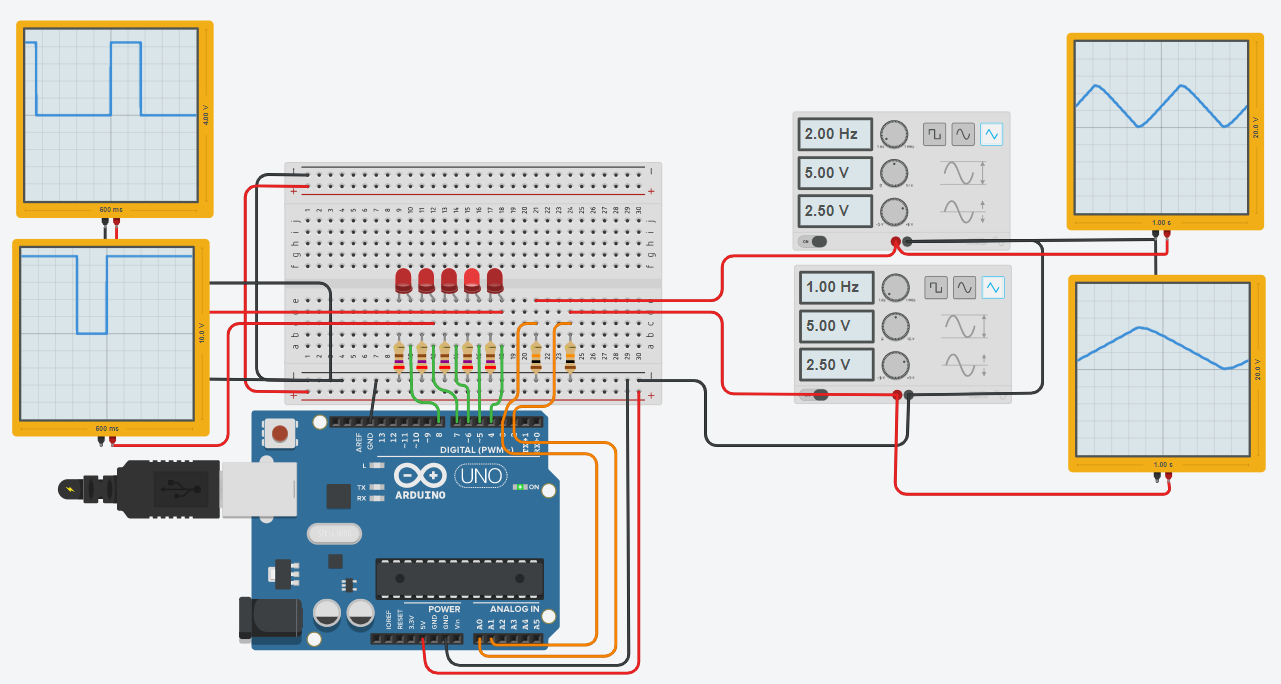
\includegraphics[width=0.8\linewidth]{Fig2.png}
	\caption{Esquema de conexión del Arduino, Generador de funciones y Osciloscopio}
	\label{fig:fig2}
\end{figure}


El código del Anexo B implementa las funciones lógicas AND, OR. Un repaso de como implementar funciones en C se muestra en \href{https://aprendiendoarduino.wordpress.com/2016/11/16/funciones-definidas-por-usuario-2/}{este enlace.} 

\subsubsection{Conteste las preguntas:}

Guarde los datos del puerto serial en un archivo .TXT e importelos en MS EXCEL para graficar los datos.
Se recomienda utilizar el monitor serial de MS CODE STUDIO dado que este permite salvar los datos.
¿Se logra apreciar las señales triangulares y digitales?
¿Las gráficas de las señales digitales de entrada y salida cumplen las tablas de verdad de las conectivas lógicas?
¿Cual es el voltaje de entrada en bajo máximo $V_{IL} max$?,
¿Cual es el voltaje de entrada en alto mínimo $V_{IH} min$?,
¿Cual es el error que presenta las mediciones de los voltajes ?,
¿Si desea un error de $\pm1$ mV, de cuantos bits debe ser el ADC?¿Explique?
\chapter{Programación de funciones combinacionales.}

\section{\obj}
\capacidad
\begin{itemize}
    \item  Programar funciones booleanas combinacionales en Arduino.
    \item  Verificar la compuertas NAND y NOR son en si mismas un conjunto Universal, equivalentes a el conjunto de conectivas lógicas OR, AND y NOT.
    \item Verificar que a partir de los mintérminos de una expresión lógica se obtienen los circuitos con compuertas NAND y de los maxtérminos, los circuitos con compuertas NOR.
    \item Verificar que para obtener la solución mínima de un circuito lógico, es necesario sintetizar los circuitos tanto por mintérminos como por maxtérminos. 
    \item Programar multiplexores $4\times1$ y $8\times1$.
\end{itemize} 


\section{\mat}
\begin{itemize}
    \item 1 Arduino UNO o equivalente: MEGA o ESP32.
    \item 1 Multímetro.
    \item 10 Resistencias de 270 o 330 $\Omega$.
    \item 5 Resistencias de 1k$\Omega$.
    \item 10 interruptores pulsadores.
    \item 1 Protoboard.
    \item 10 Diodes emisor de luz (LEDs).
    \item 1 Computadora portátil.
\end{itemize} 

\section{Marco de referencia}

Un circuito combinacional digital es un circuito que produce una o varias salidas en función de sus entradas actuales. Es decir, no mantiene ningún estado interno y su salida depende exclusivamente de sus entradas en el momento actual.
Existen muchas formas de implementar circuitos combinacionales, a partir de contactos eléctricos, válvulas neumáticas, transistores, software, etc. Sin embargo cualquier circuito lógico combinacional se puede expresar mediante cuatro formas equivalentes que describen su funcionamiento: ecuación lógica, tabla de verdad, diagrama de tiempo, y circuito eléctrico. 
Puede encontrar información adicional en el siguiente enlace \href{https://es.wikipedia.org/wiki/Sistema_combinacional}{https://es.wikipedia.org/wiki/Sistema\_combinacional}.   

\subsection{Implementan de expresiones Booleanas }

Un circuito combinacional  puede ser representado de distintas formas, pero la más común es mediante una ecuación lógica, por ejemplo: 
\begin{equation}
\label{Ec1}
F(a,b,c)=a\cdot b+\bar{a}\cdot \bar{b}\cdot c
\end{equation}

La expresión anterior posee una representación en suma de productos (SDP), puede ser implementada en C de la siguiente forma:

		 \begin{lstlisting}[language=Arduino,numbers=none, showstringspaces=false]
		bool F(bool a,bool b,bool c){
			return  (a && b) || (!a && !b && c);
		}
		\end{lstlisting} 

Existen ocho formas estándar de implementar la ecuación \eqref{Ec1} digital-mente y por consecuencia en software . Otras maneras de implementar las funciones lógicas  son con el producto de sumas (PDS), las implementaciones a dos niveles  NAND/NAND y NOR/NOR, todas las implementaciones deben arrojar los mismos resultados.

Por otra parte, la ecuación \eqref{Ec1} es equivalente a la expresión booleana  NAND/NAND si se niega dos veces y se aplica el \href{https://es.wikipedia.org/wiki/Leyes_de_De_Morgan}{Teorema de Morgan}.


\begin{align}
\label{Ec2}
F(a,b,c)&=a\cdot b+\bar{a}\cdot \bar{b} \cdot c \\
F(a,b,c)&=\overline{\overline{a\cdot b+\bar{a}\cdot \bar{b}\cdot c}} \\  \label{Ec3}
F(a,b,c)&=\overline{\overline{a\cdot b}\cdot\overline{\bar{a}\cdot \bar{b}\cdot c}}
\end{align}


Notece que la ecuacion \eqref{Ec3} necesita conectivas lógicas (funciones) de 2 y 3 entradas. Esto no es un problema cuando se implementa en SOFTWARE, pero sí se requiere hacer una implementación fisica hay que aplicar el Algebra Booleana para dejar la expresión en términos de conectivas de solamente dos entradas. Lo que se hace es que el término de tres literales, le aplicamos una doble negación tal como sigue.

\begin{eqnarray}
\label{Ec5}
F(a,b,c)=\overline{\overline{a\cdot b}\cdot\overline{\overline{\overline{\bar{a}\cdot \bar{b}}}\cdot c}} 
\end{eqnarray}

La expresión \eqref{Ec5} se encuentra en términos de conectivas NAND de dos entradas y se puede implementar en ARDUINO  de la siguiente forma:
{\footnotesize 
\begin{lstlisting}[language=Arduino,numbers=none, showstringspaces=false]
bool F(bool a, bool b, bool c){
	bool result = false;
	result = NAND(NAND(a,b),NAND(NAND(NAND(NAND(a,true),NAND(b,true)),true),c));
	return result;
}
\end{lstlisting} 
}
donde la NAND de dos entradas es:

		\begin{lstlisting}[language=Arduino,numbers=none, showstringspaces=false]
		bool NAND(bool x, bool y){
			return !(x && y);
		}
		\end{lstlisting}

\subsection{Multiplexores y Decodificadores}

Un \href{https://es.wikipedia.org/wiki/Multiplexor}{multiplexor} (Mux) es un circuito combinacional con $2^{n}$ entrada, más $n$  entradas selectoras o de control y una salida. Este circuito combinacional selecciona con las $n$ entradas control,  el valor booleano de una entrada entre $\left[ 0,2^{n}-1\right]$ y coloca dicho valor en la salida. La ecuación general de cualquier multiplexor es la siguiente,

\begin{equation}
MUX=\sum_{i=0}^{2^{n}-1} I_{i}\cdot \mathbb{S}_i
\end{equation}
donde $\mathbb{S}_i$  es la $i$-ésima permutacion de las entradas de selección. A modo de ejemplo un Mux $2 \times 1$
 posee dos entradas digitales, una de control y una salida. Un Mux $4 \times 1$ posee cuatro entradas digitales, dos de control y una salida, Un Mux $8 \times 1$ posee ocho entradas digitales, tres de control y una salida.
 
La ecuación de un Mux $4 \times 1$ es la siguiente,

\begin{equation}
	F(I_0,I_1,I_2,I_3,S_1,S_0)=I_0\bar{S_1}\bar{S_0}+I_1\bar{S_1}S_0+I_2S_1\bar{S_0}+I_3S_1S_0
\end{equation} 

El código para implementar dicho multiplexor es similar al siguiente,
{\footnotesize 
\begin{lstlisting}[language=Arduino,numbers=none, showstringspaces=false]
bool F(bool I0,bool I1,bool I2,bool I3,bool S1,bool S0){
	return (I0&&!S1&&!S0 || I1&&!S1&&S0 || I2&&S1&&!S0 || I3&&S1&&S0) ;
}
\end{lstlisting}
}
Los circuitos que realizan función inversa del multiplexor se  llama \href{https://es.wikipedia.org/wiki/Demultiplexor}{Demultiplexores}  y usualmente tiene una entrada digital más $n$ entradas de selección y $2^{n}$ salidas digitales.

Otro ejemplo de circuito combinacional son los \href{URL}{Decodificadores} y \href{https://es.wikipedia.org/wiki/Codificador}{Codificadores}.  Un codificador es un circuito combinacional con $2^{n}$ entradas y $n$ salidas, cuya misión es presentar en la salida el código binario correspondiente a la entrada activada. Mientras que un decodificador hace el trabajo inverso, recibe un código binario y lo transforma en cualquier otro código, ya sea  binarios como el Gray o exceso 3; o otras reprentaciones numericas: octal, decimal, hexagecimal. La figura \ref{fig:decoderexample} muestra la implementan digital de un decodificador de 2 a 4 líneas, la tabla de verdad del circuito y las ecuaciones características de cada salida. 
\begin{figure}
	\centering
	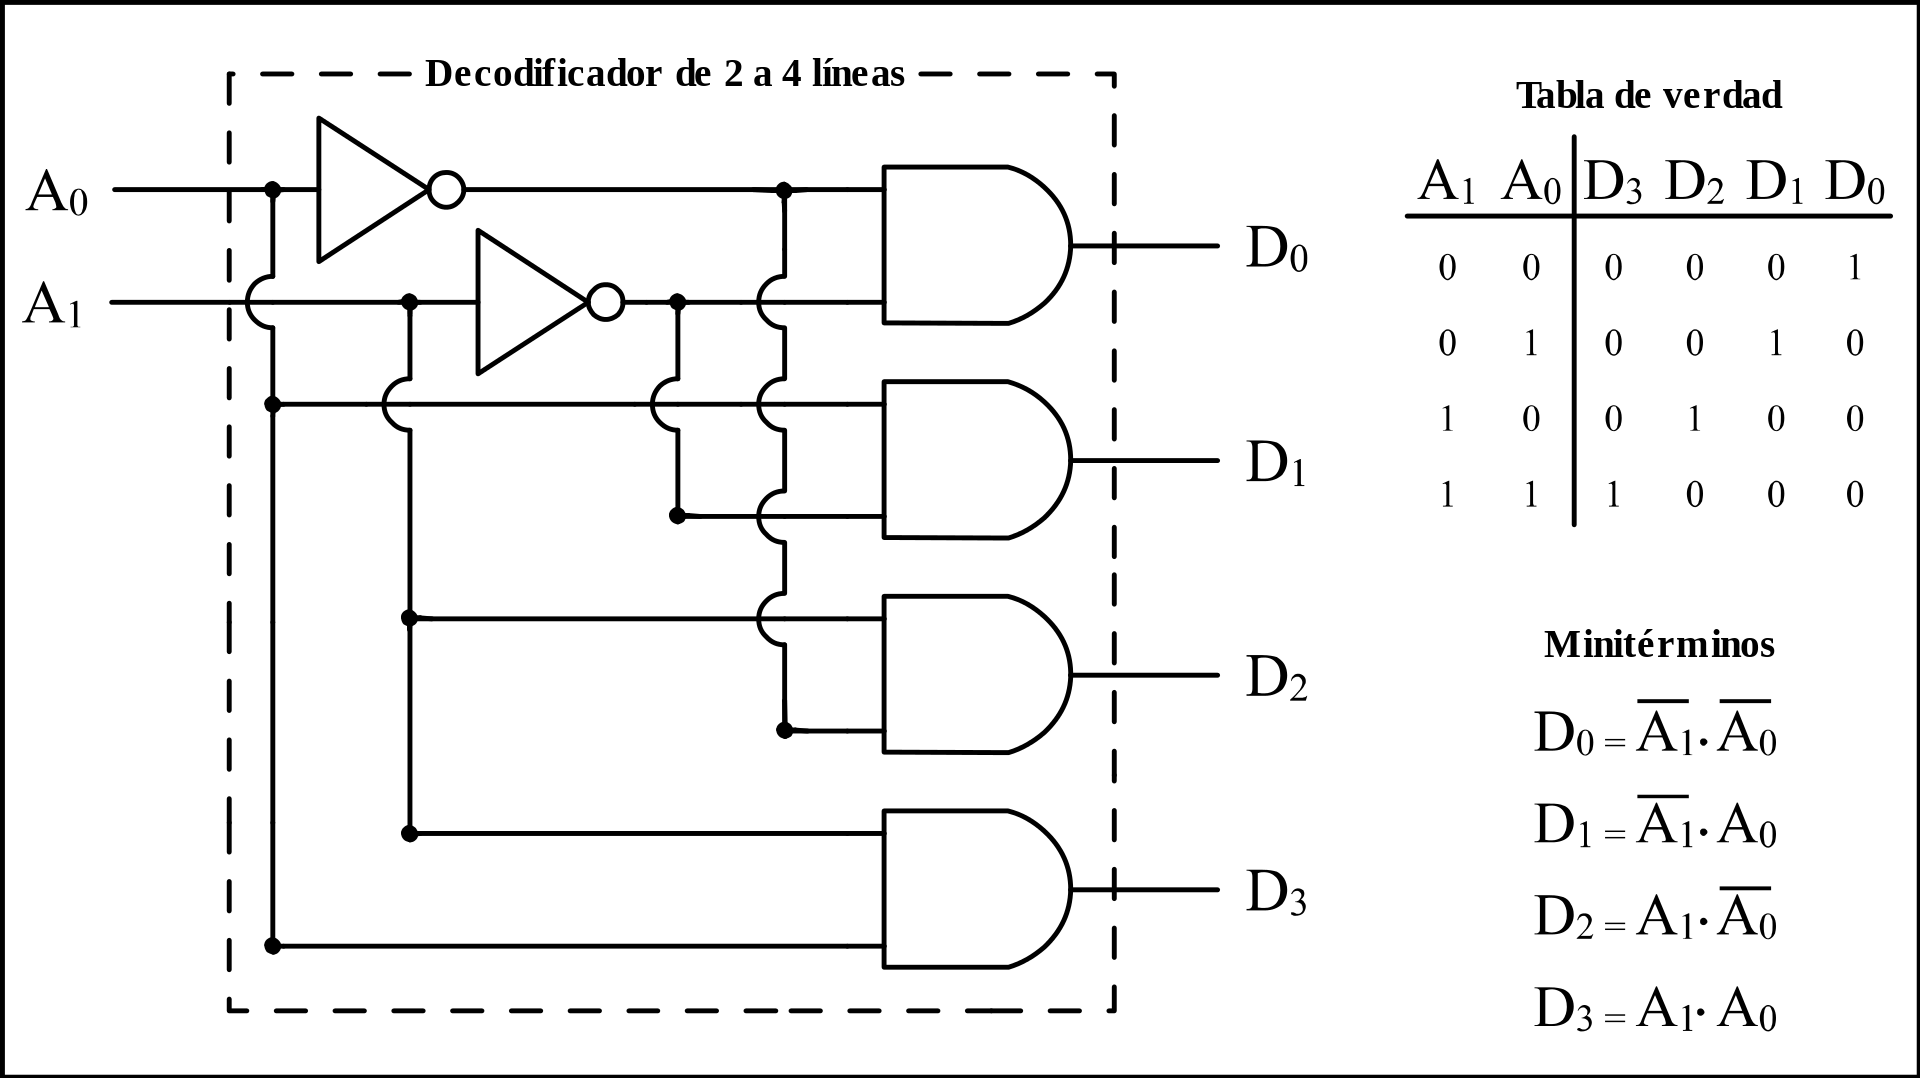
\includegraphics[width=0.7\linewidth]{Decoder_Example.png}
	\caption{Decodificador de código binario de dos bits a cuatro líneas de salida.  }
	\label{fig:decoderexample}
\end{figure}

Una posible implementación para Arduino de este decodificador es la siguiente.

\begin{lstlisting}[language=Arduino,numbers=none, showstringspaces=false]
	byte  DECO (bool A0, bool A1)
	{
		int i=0;
		bool D[4]={false, false, false, false};
		byte deco=0;
	
		D[0]=!A1 && !A0;
		D[1]=!A1 && A0;
		D[2]=A1 && !A0;
		D[3]=A1 && A0;
	
		for (i=0; i<sizeof(D);i++)
		{
			bitWrite(deco, i, D[i]);
		}
	return deco;
	}
\end{lstlisting}
  
\section{Metodología}

Este laboratorio tiene una duración de 4 lecciones, repartidas en dos semanas. Los estudiantes deben mostrar durante las clases programadas las tres actividades propuestas. Deben recabar fotografías y resultados de los equipos de medición para elaborar las evidencias. Las evidencias se subirán al TecDigital la semana siguiente finalizadas las actividades.

\section{Práctica en Clase}

\subsection{Actividad 1}

Programe en Arruino una lógica combinacional que resuelva el siguiente problema:
\begin{itemize}
    \item En una planta industrial se desea automatizar un motor y una alarma de acuerdo a 4 sensores llamados $a$, $b$, $c$ y $d$ 
    \item La señal del motor se representa por la función lógica $f1$, y se activará  cuando los sensores $a$ y $b$ estén encendidos, o cuando los sensores $b$ y $d$ estén encendidos, o cuando los sensores $a$, $c$ y $d$ están encendidos.
    \begin{equation*}
        f1 = ab + bd + acd
    \end{equation*}
    \item La señal de  alarma se representa con la función lógica $f2$, y se activará siempre que estén todos los sensores apagados excepto $a$ o todos apagados excepto $c$ o estén encendidos $c$ y $d$ y el resto apagados. También la alarma se enciende cuando todos los sensores están encendidos o cuando están todos encendidos excepto $d$ o todos encendidos excepto $c$.
    \begin{equation*}
        f2 = a\bar{b}\bar{c}\bar{d} + \bar{a}\bar{b}c\bar{d} + \bar{a}\bar{b}cd + abcd + abc\bar{d} + ab\bar{c}d
    \end{equation*}
    \begin{equation*}
        f2 = a\bar{b}\bar{c}\bar{d} + \bar{a}\bar{b}c + abc + abd
    \end{equation*}
    \item Los pines $\left\lbrace 2,3,4,5\right\rbrace$ serán las entradas digitales $\left\lbrace a,b,c,d\right\rbrace$.
    \item Los pines $\left\lbrace 6,7,8\right\rbrace $ se reservan para $f1$. Se deben implementar tres funciones: la suma de productos $(SDP)$, el producto de sumas $(PDS)$ y la función resuelta por conectivas $NAND/NAND$. 
    \begin{align*}
        &f1_{SDP} = ab + bd + acd\\
        &f1_{PDS} = (a+b)\cdot (a+d)\cdot (b+d)\cdot (b+c)\\
        &f1_{NAND/NAND} = \overline{\overline{ab} \cdot \overline{bd} \cdot \overline{acd}}
    \end{align*}
    \item Los pines $\left\lbrace 9,10,11\right\rbrace $ se reservan para $f2$. Se deben implementar tres funciones: la suma de productos $(SDP)$, el producto de sumas $(PDS)$ y la función resuelta por conectivas $NOR/NOR$.
    \begin{align*}
        &f2_{SDP} = a\bar{b}\bar{c}\bar{d} + \bar{a}\bar{b}c + abc + abd\\
        &f2_{PDS} = (a+c)\cdot (a+\bar{b})\cdot(b+c+\bar{d})\cdot(\bar{b}+c+d)\cdot (\bar{a}+b+\bar{c})\\
        &f2_{NOR/NOR} = \overline{\overline{(a+c)}\cdot \overline{(a+\bar{b})}\cdot \overline{(b+c+\bar{d})} \cdot \overline{(\bar{b}+c+d)} \cdot \overline{(\bar{a}+b+\bar{c})}}
    \end{align*}
\end{itemize}
 
\subsubsection{Conteste las preguntas:}

¿Cómo sería el circuito digital de cada una de las funciones implementadas?
¿Como es la tabla de verdad experimental de cada salida versus la tabla teórica?


\subsection{Actividad 2}

Programe las funciones de un Multiplexor 2x1, 4x1 y 8x1.
Por otra parte, existe un circuito  combinacional que se comporta como la tabla de verdad mostrada en la Tabla \ref{tab:tv}.

\begin{table}[H]
\centering
\caption{Comportamiento esperado de la estructura lógica.}
\label{tab:tv}
\begin{tabular}{ccc}
    \toprule 
    $a$ & $b$ & $F(a,b)$ \\ 
    \midrule
    0 & 0 & $c + d$ \\ 
    0 & 1 & $\overline{c + d}$ \\ 
    1 & 0 & $\overline{c \cdot d}$ \\ 
    1 & 1 & $c \oplus d$ \\ 
    \bottomrule
\end{tabular} 

\end{table}

\subsubsection{Conteste las preguntas:}

¿El comportamiento de un multiplicador $8 \times 1$ coincide con la tabla teórica?
En la funcion Loop() , llame la función del MUX  $8 \times 1$ e ingrese parámetros $\left\lbrace a,b,c,d \right\rbrace $ de tal forma que se comporte igual que la tabla de verdad presentada en el Cuadro \ref{tab:tv}.¿Tiene el mismo comportamiento?
¿Es posible implementar la T.V. con dos MUX $4 \time 1$ y un MUX  $2 \time 1$?¿Como se implementa?

\chapter{Laboratorio: Lógica convencional, Arranque-pare sencillo y reversible.}


\section{\obj}
\capacidad
\begin{itemize}
	{\small
	 \item  Estudiar  las representaciones simbólicas normalizadas de los elementos de control eléctrico, según norma NEMA ICS 19-2002 y IEC 60617.
	 \item Seleccionar contactores y relevadores térmicos.
	 \item  Estudiar la representación gráfica del estandar NEMA ICS 19-2002 o IEC 60617. 
	 \item  Diseñar e implementar circuitos de control para arranque sencillo de un motor trifásico.
	 \item  Diseñar e implementar circuitos de control para arranque-pare reversible de un  motor trifásico.
 }
\end{itemize} 

 
\section{Equipos y materiales}
Para este laboratorio de necesitaran:
\begin{itemize}
	{\small \item 1 motor trifásico 1/2 hp de 3 puntas
	\item 1 relevador térmico
	\item 1 botón pulsar cerrado
	\item 2 botones pulsadores abiertos
	\item 1 multimetro.
}
\end{itemize}

\section{Metodología}

Este laboratorio tiene una duración de 4 lecciones, repartidas en dos semanas. Los estudiantes deben mostrar durante las clases programadas las tres actividades propuestas. Deben recabar fotografías y resultados de los equipos de medición para elaborar las evidencias. Las evidencias se subirán al TecDigital la semana siguiente finalizadas las actividades.

\section{Práctica en Clase}

\subsection{Actividad 1}

 Se desea seleccionar un arrancador térmico para dos motores que mueve una bomba de agua. El primer motor es de 100 hp, trifásico (3$\varnothing$), voltaje de línea 480 voltios, voltaje de control de 120 voltios. No se requiere gabinete. El segundo motor es de 50 hp, 3$\varnothing$, 240V, 60Hz, voltaje control 120 V, ambos a plena carga con factor de potencia 0.95 en atraso. Asuma eficiencias del motor de 86\%. Por ejemplo las bombas se usan en promedio 3 veces al día todos los días y se requiere que los contactores duren al menos 20 años. 
 
\subsubsection{Conteste las preguntas}

¿Cual sería para ambos aplicaciones el modelo de arrancador con reveladores electrónicos con falla a tierra para la marca EATON según el catalogo \href{https://www.eaton.com/content/dam/eaton/products/industrialcontrols-drives-automation-sensors/nema-contactors-and-starters-v5-t2-ca08100006e.pdf}{\textit{NEMA Contactors and Starters}}, serie Freedom?. ¿Puede explicar porque se usa el mismo contactor para ambos casos?


\subsection{Actividad 2}
  Los ingenieros Electricistas, electromecánicos y de Mantenimiento pueden diseñar sus circuitos de control eléctrico, sin embargo cada fabricante posee libros de diagramas estandarizados como el que brinda  Schneider con su documento \href{https://download.schneider-electric.com/files?p_enDocType=Catalog&p_File_Name=0140CT9201.pdf&p_Doc_Ref=0140CT9201&_ga=2.160182845.1491407618.1677858387-1733391740.1677858387}{\textit{Wiring Diagram Book}}\cite{Scheneider2}.
 
 Estudie toda la simbología NEMA, Tabla 1 y Tabla 2 de la referencia \cite{Scheneider2} y asocie los con el elementos físicos y su funcionamiento.
 Deduzca la ecuación lógica del circuito eléctrico de control, para esto use un mapa de Karnaugh o la ecuacion caracteristica del cerrojo S-R prioridad al reset.
 Realice el alambrado del circuito de control y luego del circuito de potencia del arranque sencillo de un motor trifásico de 1/2 hp.

\newpage

\begin{equation*}
    M^+ = \overline{P} \cdot \overline{Sc} \cdot (A+M)
\end{equation*}

 \begin{figure}[H]
    \centering
        \begin{tikzpicture}[circuit plc ladder,scale=1.5]
        \draw(0,0)  
        to [ncpb,l=$P$] ++ (1,0) coordinate(M1)
        to [nopb,l=$A$] ++ (1,0) coordinate(M2)
        to [esource, l=$M$] ++ (1,0)
        to [contact NC={info={$Sc$}}] ++ (1,0) coordinate(laddertopright)
        (M1) -- ++ (0,-0.5) 
        to [contact NO={info={$M$}}] ++ (1,0) -- (M2)
        ;
        \ladderrungend{1}
        \ladderpowerrails
        \end{tikzpicture}
 \end{figure}

 
\subsubsection{Conteste las preguntas:}

¿Es el circuito alambrado control a dos o tres hilos? Explique. ¿El circuito de control funcionó según la tabla de verdad?, Que pasa si se pierde una fase, como se comporta el circuito?. Que diferencia existe entre un arrancador automático y uno manual en el caso que exista un corte de flujo eléctrico? Explique.
 Hasta ahora los circuitos fueron representados según la norma NEMA, muestre el circuito de control y potencia según la simbología de la norma IEC.

\subsection{Actividad 3}

Deduzca el circuito de control de un arranque-pare-reversive. Realice el alambrado del circuito de control y luego del circuito de potencia del circuito para un trifásico de 1/2 hp.


 \begin{align*}
    F^+ &= \overline{P} \cdot \overline{R} \cdot \overline{Sc} \cdot (A_F + F) \\
    R^+ &= \overline{P} \cdot \overline{F} \cdot \overline{Sc} \cdot (A_R + R)
 \end{align*}

 \begin{figure}[H]
    \centering
        \begin{tikzpicture}[circuit plc ladder,scale=1.5]
        \draw(0,0)  
        to [ncpb,l=$P$] ++ (1,0) coordinate(AF1)
        to [nopb,l=$A_F$] ++ (1,0) coordinate(AF2)
        to [contact NC={info={$R$}}] ++ (1,0)
        to [esource, l=$F$] ++ (1,0)
        to [contact NC={info={$Sc$}}] ++ (1,0) coordinate(laddertopright)
        (AF1) -- ++ (0,-0.5) 
        to [contact NO={info={$F$}}] ++ (1,0) -- (AF2)
        (M1) -- ++ (0,-2) coordinate(AR1)
        to [nopb,l=$A_R$] ++ (1,0) coordinate(AR2)
        to [contact NC={info={$F$}}] ++ (1,0)
        to [esource, l=$R$] ++ (1,0) -- ++ (0,2)
        (AR1) -- ++ (0,-0.5) 
        to [contact NO={info={$R$}}] ++ (1,0) -- (AR2)
        ;
        \ladderrungend{1}
        \ladderpowerrails
        \end{tikzpicture}
 \end{figure}

\subsubsection{Conteste las preguntas:} 

 ¿El circuito de control funcionó según la tabla de verdad?, ¿Que pasa si se presionan los botones pulsadores de arranque hacia la derecha y arranque hacia la izquierda al mismo tiempo? Explique usando el concepto de enclavamiento. 
 Muestre el circuito de control y potencia según la simbología de la norma IEC.




\chapter{Laboratorio:  Arranques a tensión reducida y circuitos temporizados.}

\section{\obj}
\capacidad
\begin{itemize}
	{\small
	 \item Diseñar un circuito secuencial temporizado que permita arrancar un motor en tensión reducida utilizando el método de estrella delta.
    \item  Diseñar un circuito secuencial temporizado que permita arrancar un motor mediante auto-transformador.
    \item  Diseñar un circuito secuencial temporizado que permita arrancar en cascada dos motores y apagarlos en cascada. 
	 \item Alambrar el circuito de control y potencia.
	 \item Detectar fallas en circuitos alambrados con lógica cableada.
	 
 }
\end{itemize} 

 
\section{Equipos y materiales}
Para este laboratorio de necesitaran:
\begin{itemize}
	{\small \item 2 motor trifásico 1/2 hp de 3 puntas.
	\item 1 motor trifásico 1/2 hp de 6 puntas.
	\item 2 relevadores térmico.
	\item 4 contactores.
	\item 1 botón pulsar cerrado.
	\item 2 botones pulsadores abiertos.
	\item 1 temporizador On-Delay.
	\item 1 temporizador Off-Delay.
	\item 1 amperimetro de gancho con medición INRUSH.
	\item 1 Analizador de señales Fluke 143B
}
\end{itemize}

\subsection{Arranque a tensión reducida}

Los arranques a tensión reducida buscan reducir el voltaje que alimenta los devanados estatóricos para que en el momento del arranque la corriente de línea se reduzca.

El arranque por autotranformador, utilizado en motores trifásicos de inducción jaula de árdilla de tres terminales, permite reducir tanto el voltaje de línea como la corriente de linea que consume el motor. Si la relacion de tranformacion es $a=V_{out}/V_{in}$, donde $V_{out}$ es el voltaje hacia el motor y $V_{in}$ es el voltage de la red. La corriente de línea antes del autotransformador es $I_{linea} = a^{2}\cdot I_{arr}$, donde $I_{arr}$ es la corriente de arranque a tensión plena. La Figura \ref{fig:control-auto-transformador} muestra el circuito de potencia y control para el arranque por auto-transformador.

Los motores trifásicos de indución jaula de ardilla de seis puntas se pueden arrancar realizando una reconfiguración de su devanado. Durante el régimen transitorio  sus devanados se alambran en estrella ($\leftthreetimes$) y cuando su velocidad alcanza el 80\% aproximadamente se realiza la re-conexión en delta ( $\Delta$) de los devanados. Esto permiten reducir el voltaje en $\sqrt{3}$ y la corriente de arranque se reduce a un tercio de la original. La Figura \ref{fig:potencia-estrella-delta} muestra el circuito de potencia para el arranque $\leftthreetimes-\Delta$.

\section{Metodología}

Este laboratorio tiene una duración de 4 lecciones, repartidas en dos semanas. Los estudiantes deben mostrar durante las clases programadas las tres actividades propuestas. Deben recabar fotografías y resultados de los equipos de medición para elaborar las evidencias. Las evidencias se subirán al TecDigital la semana siguiente finalizadas las actividades.

\section{Práctica en Clase}

\subsection{Actividad 1}

Realice un arranque-pare secuencial para dos motores trifásicos de tres puntas. Mida la corriente de arranque y la tensión de alimentación del motor.

\begin{figure}[H]
\centering
    \begin{tikzpicture}[circuit plc ladder,scale=1.3]
    \draw(0,0)  
    to [ncpb,l=$P$] ++ (1,0) coordinate(A1) 
    to [nopb,l=$A$] ++ (1,0) coordinate(A2) 
    to [esource, l=$M_1$] ++ (1,0) coordinate(A3) 
    to [contact NC={info={$S_{c1}$}}] ++ (1,0) 
    to [contact NC={info={$S_{c2}$}}] ++ (1,0) coordinate(laddertopright)
    (A1) -- ++ (0,-0.5) 
    to [contact NO={info={$M_1$}}] ++ (1,0) -- (A2)
    (A2) -- ++ (0,-1)
    to [esource, l=$T_{on}$] ++ (1,0) -- ++ (0,1)
    (A2) -- ++ (0,-2)
    to [esource, l=$T_{off}$] ++ (1,0) -- ++ (0,1)
    (0,-3) -- ++ (1,0)
    to [contact NO={info={$T_{on}$}}] ++ (1,0)
    to [esource, l=$M_2$] ++ (1,0) -- ++ (0,1)
    (0,-4) 
    to [contact NO={info={$M_2$}}] ++ (1,0)
    to [contact NO={info={$T_{off}$}}] ++ (1,0) -- ++ (0,1)
    ;
    \ladderrungend{5}
    \ladderpowerrails
    \end{tikzpicture}
    \caption{Circuito de control: arranque-pare secuencial de dos motores}
    \label{fig:control-secuencial}
\end{figure}

\begin{figure}[H]
\centering
    \begin{circuitikz}[cute inductors,scale=0.7]
    \node[esourceshape,name=motor1] at (8,-2){};
    \node[esourceshape,name=motor2] at (8,-8){};
    \draw
    (0,0) node[left]{$L_1$} 
    --++ (1.5,0) coordinate(L11) -- ++ (0.5,0)
    to [C,l=$M_1$] 
    ++ (2,0) to [wfuse,l=$S_{c1}$] ++ (2,0) -- (motor1.120)
    (0,-2) node[left]{$L_2$} 
    --++ (1,0) coordinate(L21) -- ++ (1,0)
    to [C,l=$M_1$] 
    ++ (2,0) to [wfuse,l=$S_{c1}$] ++ (2,0) -- (motor1.180)
    (0,-4) node[left]{$L_3$} 
    --++ (0.5,0) coordinate(L31) -- ++ (1.5,0)
    to [C,l=$M_1$] 
    ++ (2,0) to [wfuse,l=$S_{c1}$] ++ (2,0) -- (motor1.240)
    (L11) 
    to[short,*-] 
    ++ (0,-6) -- ++ (0.5,0) 
    to [C,l=$M_2$] 
    ++ (2,0) to [wfuse,l=$S_{c2}$] ++ (2,0) -- (motor2.120)
    (L21) 
    to[short,*-] 
    ++ (0,-6) -- ++ (1,0) 
    to [C,l=$M_2$] 
    ++ (2,0) to [wfuse,l=$S_{c2}$] ++ (2,0) -- (motor2.180)
    (L31) 
    to[short,*-] 
    ++ (0,-6) -- ++ (1.5,0) 
    to [C,l=$M_2$] 
    ++ (2,0) to [wfuse,l=$S_{c2}$] ++ (2,0) -- (motor2.240)
    (motor1.center) node{$M$}
    (motor2.center) node{$M$}
    ; 
    
    \end{circuitikz}
    \caption{Circuito de potencia: arranque-pare secuencial de dos motores}
    \label{fig:potencia-secuencial}
\end{figure}


 
\subsubsection{Conteste las preguntas}

¿Puede mostrar el circuito de control para ambas variantes y las ecuaciones lógicas?
¿Puede mostrar el diagrama de tiempos (oscilograma) del funcionamiento de cada bobina, y su relación con los eventos?
¿El circuito implementado funciona según lo planeado? ¿Cuanto es la corriente de arranque medida con el FLUKE 143B?

\subsection{Actividad 2}
 
 Realice un arranque por auto-transformador para un motor trifásico de tres puntas. Mida la corriente de arranque  y la tensión de alimentación del motor.

\begin{figure}[H]
\centering
    \begin{circuitikz}[cute inductors]
    \node[esourceshape,name=motor] at (7,-4){};
    \draw
    (0,0) node[left]{$L_1$}
    to [C,l=$G$] ++ (2,0) -- ++ (1,0) coordinate(top)
    (0,-4) node[left]{$L_2$}
    to [C,l=$G$] ++ (2,0) -- ++ (1,0) coordinate(mid)
    (0,-8) node[left]{$L_3$}
    to [C,l=$G$] ++ (2,0) -- ++ (1,0) coordinate(bot)
    (top)
    to [L,name=L1] ++ (0,-3)
    to [C,l=$E$] (mid)
    to [C,l=$E$] ++ (0,-1)
    to [L,name=L2] ++ (0,-3)
    (L1.midtap) -- ++ (1,0) 
    to [C,l_=$D$] ++ (0,1.5) -- (top)   
    (L2.midtap) -- ++ (1,0) 
    to [C,l_=$D$] ++ (0,-1.5) -- (bot) 
    (L1.midtap) node[below,xshift=22]{$H_3 H_2$} ++ (1,0) to [wfuse,l=$S_{c}$] ++ (2,0) -- (motor.120)
    (L2.midtap) node[above,xshift=22]{$H_3 H_2$} ++ (1,0) to [wfuse,l=$S_{c}$] ++ (2,0) -- (motor.240)
    (mid) --++ (1,0) to [wfuse,l=$S_{c}$] ++ (2,0) -- (motor.180)
    (motor.center) node{$M$}
    (L1.core west) node[left,xshift=-8]{$H_1$}
    (L1.core east) node[left,xshift=-8]{$H_5$}
    (L2.core west) node[left,xshift=-8]{$H_1$}
    (L2.core east) node[left,xshift=-8]{$H_5$}
    ;
    \end{circuitikz}
    \caption{Circuito de potencia: arranque por auto-transformador}
    \label{fig:potencia-auto-transformador}
\end{figure}

\begin{figure}[H]
\centering
    \begin{tikzpicture}[circuit plc ladder,scale=1.3]
    \draw(0,0)  
    to [ncpb,l=$P$] ++ (1,0) coordinate(A1)
    to [nopb,l=$A$] ++ (1,0) coordinate(A2)
    to [contact NC={info={$Sc$}}] ++ (1,0)
    to [esource, l=$G$] ++ (1,0) coordinate(laddertopright)
    (A1) -- ++ (0,-0.5) 
    to [contact NO={info={$G$}}] ++ (1,0) -- (A2)
    ;
    \ladderrungend{1}
    \draw(0,0)
    to [contact NO={info={$G$}}] ++ (1,0) coordinate(T1) --++ (2,0)
    to [esource, l=$T_{on}$] ++ (1,0)
    (T1) -- ++ (0,-1)
    to [contact NC={info={$T_{on}$}}] ++ (1,0)
    to [contact NC={info={$D$}}] ++ (1,0)
    to [esource, l=$E$] ++ (1,0)
    (T1) ++ (0,-1) --++ (0,-1)
    to [contact NO={info={$T_{on}$}}] ++ (1,0)
    to [contact NC={info={$E$}}] ++ (1,0)
    to [esource, l=$D$] ++ (1,0)
    ;
    \ladderrungend{3}
    \ladderpowerrails
    \end{tikzpicture}
    \caption{Circuito de control: arranque por auto-transformador}
    \label{fig:control-auto-transformador}
\end{figure}

 
 
\subsubsection{Conteste las preguntas:}

¿Cual es la corriente de arranque del motor según su dato de placa y letra de código? ¿Cuanto es la corriente de arranque medida con el FLUKE 143B? ¿Cuanto se redujo la corriente en el arranque?¿Se cumple la ecuación $I_{linea} = a^{2}\cdot I_{arr}$ ?

\subsection{Actividad 3}

Realice un arranque pare reversible para un motor que arranca en estrella-delta. Es decir, el motor debe arrancar en estrella-delta hacia la derecha, o puede arrancar en estrella-delta hacia la izquierda. Cuando se presiona el botón de pare o sobrecarga este se detiene. Solo se requiere un temporizador tipo On-Delay.

\begin{figure}[H]
\centering
    \begin{circuitikz}[cute inductors,scale=0.7]
    \draw
    (0,0) node[left]{$L_1$} 
    --++ (1.5,0) coordinate(L11) -- ++ (0.5,0)
    to [C,l=$F$] 
    ++ (2,0) -- ++ (1.5,0) coordinate(L12) -- ++ (0.5,0) coordinate(L13)
    (0,-2) node[left]{$L_2$} 
    --++ (1,0) coordinate(L21) -- ++ (1,0)
    to [C,l=$F$] 
    ++ (2,0) -- ++ (1,0) coordinate(L22) -- ++ (1,0) coordinate(L23) 
    (0,-4) node[left]{$L_3$} 
    --++ (0.5,0) coordinate(L31) -- ++ (1.5,0)
    to [C,l=$F$] 
    ++ (2,0) -- ++ (0.5,0) coordinate(L32) -- ++ (1.5,0) coordinate(L33)
    (L31) 
    to[short,*-] 
    ++ (0,6) -- ++ (1.5,0) 
    to [C,l=$R$] 
    ++ (2,0) -- ++ (0.5,0) 
    to[short,-*]
    (L32)
    (L21) 
    to[short,*-] 
    ++ (0,6) -- ++ (1,0) 
    to [C,l=$R$] 
    ++ (2,0) -- ++ (1.5,0) 
    to[short,-*]
    (L12)
    (L11) 
    to[short,*-] 
    ++ (0,6) -- ++ (0.5,0) 
    to [C,l=$R$] 
    ++ (2,0) -- ++ (1,0) 
    to[short,-*]
    (L22)
    (L13) to[wfuse,l=$S_{c}$] ++ (2,0) --++ (4,0) node[above]{$6$}
    to [L,name=L1,*-*]
    ++ (2,0) node[above]{$3$} -- ++ (3.5,0) coordinate(L14) -- ++ (0.5,0) coordinate(L15)
    (L23) to[wfuse,l=$S_{c}$] ++ (2,0) --++ (4,0) node[above]{$5$}
    to [L,name=L2,*-*]
    ++ (2,0) node[above]{$2$} -- ++ (3,0) coordinate(L24) -- ++ (1,0) coordinate(L25)
    (L23) ++ (7,0) node[yshift=-75]{motor} circle (3)
    (L33) to[wfuse,l=$S_{c}$] ++ (2,0) --++ (4,0) node[above]{$4$}
    to [L,name=L3,*-*]
    ++ (2,0) node[above]{$1$} -- ++ (2.5,0) coordinate(L34) -- ++ (1.5,0) coordinate(L35)
    (L32) 
    ++ (4,0) 
    to[short,*-]
    ++ (0,6) -- ++ (3.5,0)
    to[C,l=$D$]
    ++ (2,0) -- ++ (3,0)
    to[short,-*] 
    (L24)
    (L22) 
    ++ (4,0) 
    to[short,*-]
    ++ (0,6) -- ++ (3,0)
    to[C,l=$D$]
    ++ (2,0) -- ++ (3.5,0)
    to[short,-*] 
    (L14)
    (L12) 
    ++ (4,0) 
    to[short,*-]
    ++ (0,6) -- ++ (2.5,0)
    to[C,l=$D$]
    ++ (2,0) -- ++ (2.5,0)
    to[short,-*] 
    (L34)
    (L15)
    to[C,l=$E$] 
    ++ (2,0) -- ++ (1,0)
    to[short,-*] ++ (0,-2)
    (L25)
    to[C,l=$E$] 
    ++ (2,0) -- ++ (1,0)
    (L35)
    to[C,l=$E$] 
    ++ (2,0) -- ++ (1,0)
    to[short,-*] ++ (0,2)
    ;
    \end{circuitikz}
    \caption{Circuito de potencia: arranque Estrella-Delta Reversible}
    \label{fig:potencia-estrella-delta}
\end{figure}

\begin{figure}[H]
\centering
    \begin{tikzpicture}[circuit plc ladder,scale=1.3]
    \draw(0,0)  
    to [ncpb,l=$P$] ++ (1,0) coordinate(AF1)
    to [nopb,l=$A_F$] ++ (1,0) coordinate(AF2)
    to [contact NC={info={$R$}}] ++ (1,0)
    to [esource, l=$F$] ++ (1,0) 
    to [contact NC={info={$S_c$}}] ++ (1,0) coordinate(laddertopright)
    (AF1) -- ++ (0,-0.5) 
    to [contact NO={info={$F$}}] ++ (1,0) -- (AF2)
    (AF1) -- ++ (0,-1.5) coordinate(AR1)
    to [nopb,l=$A_R$] ++ (1,0) coordinate(AR2)
    to [contact NC={info={$F$}}] ++ (1,0)
    to [esource, l=$R$] ++ (1,0) -- ++ (0,1.5)
    (AR1) -- ++ (0,-0.5) 
    to [contact NO={info={$R$}}] ++ (1,0) -- (AR2)
    (0,-4)
    to [contact NO={info={$R$}}] ++ (1,0)
    (0,-3)
    to [contact NO={info={$F$}}] ++ (1,0) coordinate(FR) -- ++ (2,0)
    to [esource, l=$T_{on}$] ++ (1,0) -- ++ (0,1.5)
    (FR) -- ++ (0,-1) 
    to [contact NC={info={$T_{on}$}}] ++ (1,0)
    to [contact NC={info={$D$}}] ++ (1,0)
    to [esource, l=$E$] ++ (1,0)
    (FR) ++ (0,-1) --++ (0,-1)
    to [contact NO={info={$T_{on}$}}] ++ (1,0)
    to [contact NC={info={$E$}}] ++ (1,0)
    to [esource, l=$D$] ++ (1,0) -- ++ (0,2)   
    ;
    \ladderrungend{6}
    \ladderpowerrails
    \end{tikzpicture}
    \caption{Circuito de control: arranque Estrella-Delta Reversible}
    \label{fig:control-estrella-delta}
\end{figure}

\subsubsection{Conteste las preguntas:} 

 ¿Como es el circuito implementado? ¿Cuanto es la corriente de arranque medida con el FLUKE 143B? ¿Como es el diagrama de tiempos de cada bobina? ¿La corriente de arranque se redujo un tercio del arranque a plena tensión? 




\chapter{Laboratorio:  Programación de variadores de frecuencia y arrancadores suaves.}

\section{\obj}
\capacidad
\begin{itemize}
	{\small
    \item  Alambrar el circuito de control y potencia del variador.
    \item  Programar un variador de frecuencia segun los requerimientos. 
	\item Alambrar el arrancador suave para un motor trifásico.
	\item Alambrar un arranque pare reversible usando un arrancador suave de un motor trifásico.
	\item Programar el variador de frecuencia.
	\item Medir el tiempo de las rampas de aceleración y desaceleración, y vincular con los parámetros programados.
 }
\end{itemize} 

 
\section{Equipos y materiales}
Para este laboratorio de necesitaran:
\begin{itemize}
	{\small \item 1 motor trifásico 1/2 hp de 3 puntas.
	\item 1 variador de frecuencia: \href{https://search.abb.com/library/Download.aspx?DocumentID=3AUA0000066143&LanguageCode=en&DocumentPartId=1&Action=Launch}{ABB ACS355} o \href{https://vfds.com/content/manuals/delta/delta-vfd-el-manual.pdf}{VFD-EL}
	\item 1 arrancador suave SIEMENS RW3013.
	\item 2 contactores.
	\item 1 botón pulsar cerrado.
	\item 2 botones pulsadores abiertos.
	\item 3 interruptores N.O.
	\item 1 amperimetro de gancho con medición INRUSH.
	\item 1 analizador de señales trifásico FLUKE 143B.
}
\end{itemize}

\section{Metodología}

Este laboratorio tiene una duración de 4 lecciones, repartidas en dos semanas. Los estudiantes deben mostrar durante las clases programadas las tres actividades propuestas. Deben recabar fotografías y resultados de los equipos de medición para elaborar las evidencias. Las evidencias se subirán al TecDigital la semana siguiente finalizadas las actividades.

\section{Práctica en Clase}

\subsection{Actividad 1}

Suponga que el arrancador suave es para un motor de una cinta transportadora que puede operar en ambos sentidos. Según el manual del \href{https://support.industry.siemens.com/dl/files/095/38752095/att_1310813/v1/Manual_softstarter_3RW30_3RW40_es-MX.pdf}{SIRIUS 3RW30} \cite{SIEMENS}, sección 13.1.2, seleccione el voltaje de inicio y la rampa de tiempo recomendada.
Implemente un circuito de control y potencia para que el motor arranque en dos sentidos, para esto puede usar como referencia la sección 16 de ejemplos. 
 
\subsubsection{Conteste las preguntas}

¿Puede mostrar el circuito de control del sistema?
Usando un analizador Fluke 143B  mida la corriente de arranque del motor.
¿Como son las señales de corriente y voltaje a la entrada del motor con/sin arrancador suave?
¿Cuanto tiempo tardó en aparecer el voltaje de línea en las terminales?¿Coincide con la rampa de tiempo pre-establecida?

\subsection{Actividad 2}
 

Utilizando el manual del variador, encuentre el código que re-inicial el VDF a sus valores de fábrica.
Luego ingrese los parámetros descritos en la sección 3.3 asociados al voltaje, corriente nominal y frecuencia base del motor.
Posteriormente seleccione un modo de entrada que permita operar el motor en ambos sentidos mediante cableado externo.
Programe rampas de aceleración entre las frecuencias mínimas y máximas de 20 segundos y de desaceleración de 30.
Programe siete frecuencias en el VDF, asumiendo torque constante en vacío,de tal forma que en el eje del motor se midan las velocidades de la Tabla \ref{Tab:velocidades}.

\begin{table}[H]
	\centering  
	\caption{Velocidades solicitadas}
	\label{Tab:velocidades}
	\begin{tabular}{|c|c|}
		\hline 
		Velocidad	&	Rev/min	\\	\hline 
		
		0	&	900	  	   	 \\ 
		1	&	1050	  	   	 \\ 
		2	&	1200	  	   	 \\ 
		3	&	1350	  	   	 \\ 
		4	&	1500	  	   	 \\ 
		5	&	1650	    	 \\ 
		6	&	1800        	 \\ 
		7	&	1950     	   	 \\ 
		\hline 
	\end{tabular} 
\end{table}
 

 
\subsubsection{Conteste las preguntas:}

Realice la gráfica de voltaje en función de la frecuencia ($V=\mathfrak{F}(f)$), ¿Es como se esperaba?
Realice una tabla con las mediciones de las velocidades medidas, ¿Cuál fue el porcentaje de error relativo de cada medición?
Si se programa el variador con frecuencias calculadas con torque variable, los errores mejoran o empeoran? ¿Por qué?
¿Son las gráficas PWM a la salida del variador son como se esperan? ¿Puede mostrar un gráfico? Si se desconecta una fase de entrada en VDF, ¿que sucedió con el VDF? Mida las rampas de aceleración y desaceleración, cumple lo programado? Cuanto tarda de pasar de la velocidad 3 a la 5 y viceversa, tienen estos tiempos sentido? Que pasaría si se programan rampas de 1 segundo de aceleración y des-aceleración?
 

%\section{Informe de evidencias para el TECDIGITAL}
%
% Para cada actividad copie los resultados que se imprimieron en el puerto serial. Adicionalmente, para las actividades 2 y 3 muestre las fotografías de los circuitos.
% 
% El informe que se sube al TEC DIGITAL debe ser un archivo PDF, con las siguiente partes:
% 
% \begin{enumerate}
% 	\item Identificación del laboratorio, Autores, fecha.
% 	\item Resumen
% 	\item Objetivos
% 	\item Descripción de la actividad x.
% 	\item Evidencia fotográfica de los circuitos. 
% 	\item Evidencia de los resultados obtenidos (gráficas, tablas, imágenes, etc ).
% 	\item Análisis de las preguntas planteadas en la actividad.
% 	\item Referencias.
% \end{enumerate}
% 
% Si el laboratorio posee x actividades los pasos 4,5,6 y 7 se repiten x veces. 




\chapter{Laboratorio:  Programación con LOGO!}
	  
\section{\obj}
Este  laboratorio busca:
\begin{itemize}
	{\small
    \item Programar e implementar un arranque en Estrella -Delta usando un el relé inteligente LOGO!.
    \item Programar e implementar un alternador de dos bombas.
    \item Programar un alternador de bombas con señales de alarma y temporizadores semanales.
    \item Aprender las conexiones eléctricas de las entradas y salidas del controlador.
    \item Calcular el ciclo de trabajo de cada programa de cada programa 
 }
\end{itemize} 

 
\section{Equipos y materiales}
Para este laboratorio de necesitaran:
\begin{itemize}
	{\small \item 2 motores trifásicos 1/2 hp de 3 puntas.
		\item 1 motor trifásico de 6 puntas.
	\item 1 Logo! 230RC de Siemmens.
	\item 1 Software LOGO! Confort.
	\item 4 contactores.
	\item 1 botón pulsar cerrado.
	\item 3 botones pulsadores abiertos.
	\item 1 \href{https://cache.industry.siemens.com/dl/files/041/109741041/att_924629/v1/logo_system_manual_es-ES_es-ES.pdf}{Manual del LOGO! 8}.
	\item 1 \href{https://cache.industry.siemens.com/dl/files/807/100782807/att_924633/v1/Help_es-ES_es-ES.pdf}{Manual LOGO!Soft Comfort.}
}
\end{itemize}

\section{Metodología}

Este laboratorio tiene una duración de 4 lecciones, repartidas en dos semanas. Los estudiantes deben mostrar durante las clases programadas las tres actividades propuestas. Deben recabar fotografías y resultados de los equipos de medición para elaborar las evidencias. Las evidencias se subirán al TecDigital la semana siguiente finalizadas las actividades.

\section{Práctica en Clase}

\subsection{Actividad 1}

	El profesor realizara el programa de control para un arranque en estrella-delta en LOGO!Soft Comfort y explicará todo lo concerniente a: simulación del programa, y a la configuración de la red local (LAN), Mascara, pasarela de salida (gateway), y carga en el programa. 
	
 \subsubsection{Conteste las preguntas}
 	¿Que información brinda el comando IPCONFIG en COMMAND PROMPT de Windows?, ¿Que información brinda el comando PING?.  

\subsection{Actividad 2}


Diseñe el programa para el controlador LOGO!, que resuelva el siguiente problema.

Se necesita un alternador de bombas  para el llenado de un tanque de almacenamiento. El taque posee tres niveles, NA nivel alto, NB nivel bajo y Nivel Crítico NC, además existen 2 bombas B1 y B2. Cuando el agua activa NB la bomba B1 se activa y se apaga hasta alcanzar el nivel NA. La próxima vez que se active el sensor NB se activa la segunda bomba B2 y se apaga hasta alcanzar NA. Este ciclo se repite hasta que se presione el apagado general del sistema o se active una de las dos sobrecargas. Si el nivel crítico se presiona NC se encienden ambas bombas, además el sistema debe  recordar el orden de la alternancia. El sistema cuenta con dos botoneras para el arranque y pare general del sistema. El sistema deberá mostrar en pantalla en todo momento,  el estado de la bombas y la etapa lógica en que se encuentra el sistema.

Una vez simulada la solución, procederá a cargarla y alambrar el LOGO!. Para esto requerirá de las botoneras pulsadoras, contactores y finales de carrera que emulan los niveles de la boyas, etc. 

% \begin{figure}
%     \centering
%     \begin{circuitikz}
%     \draw (0,0)
%     to [esource, l=$F$] --++ (1,0) 
%     ;
%     \end{circuitikz}
%     \caption{Caption}
%     \label{fig:enter-label}
% \end{figure}


\subsubsection{Conteste las preguntas}

¿Puede mostrar el diagrama lógico de la solución?, ¿Puede mostrar el diagrama de la implementación con sus  ecuaciones lógicas?, ¿Puede mostar el diagrama de conexión eléctrico?.¿Cuando es el ciclo de escaneo de la solución? La ultima pregunta se contesta implementando el código que se aporta en apéndice B del manual \cite{LOGO1}.

\subsection{Actividad 3}
Diseñe el programa para el controlador LOGO!, que resuelva el siguiente problema.

La empresa \textbf{Automation Solutions} necesita controlar dos moto-bombas de forma alternada.

Las entradas del sistema son:  botón del arranque motor A, botón de paro del motor A,  presostato de confirmación del motor A, botón del arranque motor B, botón de paro del motor B,  presostato de confirmación del motor B. 

Las salidas del controlador son las señales a los contactares de la moto-bomba A y la moto-bomba B.

El sistema debe funcionar con la siguiente lógica:

\begin{itemize}
	\item Si el sistema esta en modo manual, el arranque y pare se realiza desde las botoneras. Si a los 3 segundos no existe la señal de confirmación de presión, aparece en pantalla del LOGO! un mensaje indicando que la bomba no levanta presión, y se desactiva el enclave-miento de  la señal del motor.
	\item Por otra parte, si la maneta esta en la posición de modo automático, la bomba X se enciende a las 5PM y se apaga a las 10PM. El arranque y pare de las moto-bombas es de forma alternada. Es decir, si el Lunes arranca la  moto-bomba B1, el Martes deberá arrancar la moto-bomba B2 y así sucesivamente. Si la confirmación de presión no se recibe en un lapso de 3 segundo, el sistema cambiará a la otra bomba y mostrara en pantalla el aviso del cambio.	
	\item Adicionalmente, existe un  contador que indica en pantalla del LOGO!, la cantidad de ciclos de la bomba 1 y de la bomba 2. Cuando los ciclos realizados sean igual a 10 aparecerá en pantalla un mensaje indicando : “La bomba Bx requiere mantenimiento”. En pantalla se debe indicar la etapa lógica del sistema.
\end{itemize} 




\subsubsection{Conteste las preguntas}
¿Puede mostrar el diagrama lógico de la solución?, ¿Puede mostrar el diagrama de la implementación con sus  ecuaciones lógicas?, ¿Puede mostar el diagrama de conexión eléctrico?.¿Cuando es el ciclo de escaneo de la solución? La ultima pregunta se contesta implementando el código que se aporta en apéndice B del manual \cite{LOGO1}.




\chapter{Laboratorio:  Programación de Autómatas Lógicos}


\section{Objetivos}
Este  laboratorio busca:
\begin{itemize}
	{\small
    \item Entender la implementación de la norma IEC 61131-3.
    \item Programar  de manera estructura el PLC S7-1500 usando bloques OB, FB y DB.
    \item Utilizar tres lenguajes estandarizados para la programación de bloques lógicos.
    \item Solucionar problemas comunes de automatización.
 }
\end{itemize} 

 
\section{Equipos y materiales}
Para este laboratorio de necesitaran:
\begin{itemize}
	{\small 
	\item 1 PLC SIEMENS 1500.
	\item 1 Software TIA Portal V17.
	\item 1 Computadora.
	\item 1 \href{https://support.industry.siemens.com/dl/files/056/109815056/att_1121729/v4/STEP_7_WinCC_V18_esES_es-ES.pdf}{Manual del software TIA Portal}.
	\item 1 \href{https://cache.industry.siemens.com/dl/files/384/86140384/att_1131259/v1/s71500_et200mp_manual_collection_es-ES.pdf}{Colección de Manuales S7-1500}
}
\end{itemize}

\section{Metodología}

Este laboratorio tiene una duración de 4 lecciones, repartidas en dos semanas. Los estudiantes deben mostrar durante las clases programadas las tres actividades propuestas. Deben recabar fotografías y resultados de los equipos de medición para elaborar las evidencias. Las evidencias se subirán al TecDigital la semana siguiente finalizadas las actividades.

\section{Práctica en Clase}

\subsection{Actividad 1}

	Se requiere programar un arranque estrella-delta con multiples instancias. Para realizar esta actividad, utilize el lenguaje de contactos (KOP) para programar un  estrella - delta  dentro de un Bloque de función (FB). El FB tendrá como parámetros de entrada: la señal de arranque, pare, sobre carga y tiempo del temporizador. Como señales de salida tendrá la de la bobina general, la bobina que realiza el estrella y la bobina en delta.
	
	Luego en el bloque de organizacion uno (OB1), se llama el bloque  FB multiple veces. Por ejemplo, llame el FB tres veces y ponga tiempos de arranque distintos \{3, 6, 9\} segundos al parámetro tiempo  de  cada instancia.
	
 \subsubsection{Conteste las preguntas}
  
  Si se presiona el arranque al mismo tiempo, ¿como fue diagrama de tiempos de las 9 señales?
  ¿Puede mostrar el diagrama KOP del FB y OB1 implementado?
  

\subsection{Actividad 2}

Se necesita automatizar un parque de pozos profundos, el parque posee tres pozos y y tres tanques de captación. Se desea un sistema general que inicialice y pares los tres subsistemas, es decir, cuando se presione el arranque inicien el sistema de los tres pozos y cuando se presione el pare se detengan. Cuando se active una sobrecarga de algún motor ese subsistema en específico deja de funcionar, pero los otros dos subsistemas de pozos y tanque siguen funcionando normalmente. Los subsistemas se llamarán S1, S2 y S3 respectivamente.

Cada subsistema de pozo profundo se compone de dos bombas que funcionan en alternancia, un pozo de captación y un tanque de almacenamiento. Las señales del tanque de almacenamiento indican el nivel alto \textbf{T1-Na}, y nivel bajo \textbf{T1-Nb} de agua, el pozo profundo posee también dos sensores de nivel, nivel alto \textbf{P1-Na} y nivel bajo \textbf{P1-Nb}, además existen las dos señales de salida para las dos bombas: \textbf{S1-B1} y \textbf{S1-B2}. 

EL funcionamiento del subsistema es de la siguiente forma: las bombas toman el agua del pozo y la deposita en el tanque de captación. El nivel de agua \textbf{T1-Nb} activa la bomba \textbf{S1-B1} siempre y cuando la señal de \textbf{P1-Na} este activa. La bomba \textbf{S1-B1}  se apaga hasta alcanzar el nivel \textbf{T1-Na}  o que se quede sin agua indicado por el sensor del pozo \textbf{P1-Nb}. Dicho de otra forma, si antes de alcanzar el sensor \textbf{T1-Na} se activase el nivel \textbf{PI-Nb}, se apaga la bomba. La próxima vez que se active el sensor \textbf{T1-Nb}  y este activa el sensor \textbf{P1-Na} se activa la segunda bomba \textbf{S1-B2} y se apaga hasta alcanzar \textbf{T1-Na} o \textbf{P1-Nb}.   Este ciclo se repite hasta que se presione el apagado general del sistema o se active una de las dos sobrecargas del subsistema.

Para los subsistemas 2 y 3 simplemente cambie los subindices en los sensores del tanque, pozo, bombas y sobrecargas son: \textbf{T\#-Nx}, \textbf{P\#-Nx}, \textbf{S\#-B\#}, \textbf{S\#-Sc\#}. Por ejemplo, la codificación de los sensores de nivel alto del tanque y el pozo se indica de la forma: \textbf{T3-Na} y \textbf{P3-Na}.

Cada subsistema posee un contador de número de ciclos. El valor del contador es un parámetro de entrada. Cuando se llega al valor se activa una señal de alarmar para el mantenimiento. La alarma se restablece un boton pulsador.

\begin{itemize}
	\item Realice la programación con el Gráfico de Función Secuencial de SIEMENS llamado GRAPH.
	\item Cree un Bloque de función FB1 genérico  usando el lenguaje GRAPH.
	\item Cree un Bloque de  función FB2 general en diagrama de contactos (KOP), donde se llame 3 veces al bloque anterior y  renombre todos los parametros de entrada.
	\item En el Bloque de organización OB1, inserte el bloque FB2.
	\item Verifique el funcionamiento  la solución del problema mediante simulación.
	\item Cargue el programa en el PLC S7-1500.
	\item Active el monitoreo de las entradas y salidas del PLC y su visualización en la pantalla. 
	
\end{itemize}

\subsubsection{Conteste las preguntas}

¿Como es la implementación de contadores y temporizadores en GRAPH?
¿Como se declaran los parámetros de entrada  y salida de un bloque de función (FB)?
¿Como se comportó el sistema implementado? ¿Puede mostrar el diagrama del FB1 y FB2?

\subsection{Actividad 3}

Repita la actividad 2, pero implemente el ejercicio en texto estructurado (ST), con la variante que cada bomba del pozo requiere arrancar en estrella-delta.
Para esta actividad podrá usar el FB programado en la actividad 1, y llamar este bloque múltiples veces. 
 

%\section{Informe de evidencias para el TECDIGITAL}
%
% Para cada actividad copie los resultados que se imprimieron en el puerto serial. Adicionalmente, para las actividades 2 y 3 muestre las fotografías de los circuitos.
% 
% El informe que se sube al TEC DIGITAL debe ser un archivo PDF, con las siguiente partes:
% 
% \begin{enumerate}
% 	\item Identificación del laboratorio, Autores, fecha.
% 	\item Resumen
% 	\item Objetivos
% 	\item Descripción de la actividad x.
% 	\item Evidencia fotográfica de los circuitos. 
% 	\item Evidencia de los resultados obtenidos (gráficas, tablas, imágenes, etc ).
% 	\item Análisis de las preguntas planteadas en la actividad.
% 	\item Referencias.
% \end{enumerate}
% 
% Si el laboratorio posee x actividades los pasos 4,5,6 y 7 se repiten x veces. 




%----------------------------------------------------------------------------------------
%	APPENDIX
%----------------------------------------------------------------------------------------

\appendix
\chapter{Marcos de referencia}
\section{Arduino}

Un micro-controlador es un circuito integrado pequeño que contiene un microprocesador, memoria y periféricos como entradas/salidas (IO), comunicación, almacenamiento y sensores. Estos componentes están integrados en un solo chip y pueden ser programados para controlar diferentes dispositivos y sistemas.

Entre las partes que pueden contener los micro-controladores se encuentran: 

\begin{itemize}
    \item Microprocesador: es la unidad aritmética lógica,  registros asociados y controladores  que realizan  las operaciones del sistema y es responsable de ejecutar las instrucciones del programa.
    \item Memoria: donde se almacena el programa y los datos.
    \item Entradas/Salidas (IO): permite la comunicación entre el micro-controlador y el mundo exterior.
    \item Comunicación: permite que el micro-controlador se comunique con otros dispositivos a través de diferentes protocolos como USB, Ethernet, etc.
    \item Almacenamiento: permite almacenar datos en el dispositivo, como una EEPROM o una memoria flash.
    \item Sensores: permiten medir diferentes variables ambientales como la temperatura, la humedad, la presión, etc.
\end{itemize}

Los micro-controladores tienen muchos usos, incluyendo: 
\begin{itemize}
    \item Control de motores,
    \item Automatización de procesos industriales,
    \item Dispositivos de medida y monitoreo,
    \item Control de sistemas de iluminación y calefacción,
    \item Control de sistemas de seguridad,
    \item Control de electrodomésticos y dispositivos de consumo,
    \item Control de sistemas de comunicación,
    \item Control de sistemas de vehículos,
    \item Control de robots y sistemas automatizados.
\end{itemize}
\subsection{Arduino}

El Arduino es una plataforma de desarrollo de hardware y software libre basada en un micro-controlador. La programación de Arduino se basa en el lenguaje de programación C++ y utiliza un entorno de desarrollo integrado (IDE) específico llamado Arduino IDE. El Arduino IDE es una aplicación de escritorio que se utiliza para escribir, depurar y cargar código en el micro-controlador.

El procedimiento básico de programación del Arduino es el siguiente:

\begin{enumerate}
    \item Conectar el Arduino a la computadora mediante un cable USB.
    \item Abrir el Arduino IDE y seleccionar el tipo de Arduino y la tarjeta que se va a utilizar en el menú Herramientas.
    \item Escribir el código en el editor de código del Arduino IDE, utilizando el lenguaje de programación C++.
    \item Verificar el código compilando el código utilizando el botón verde de compilación del Arduino IDE.
    \item Cargar el código en el Arduino utilizando el botón azul de carga del Arduino IDE.
    \item Observar el comportamiento del código en los pines de entrada y salida del Arduino, si es necesario realizar cambios en el código para obtener el resultado deseado.
    \item Repetir los pasos 3-6 hasta que el código funcione correctamente.
\end{enumerate}

El esquema básico de programación de Arduino utiliza dos funciones esenciales \cite{margolis2020arduino}: setup() y loop().

La función \href{https://www.arduino.cc/reference/en/language/structure/sketch/setup/}{setup()}: Es la primera función que se ejecuta cuando el Arduino se enciende o se reinicia. En esta función se configuran los pines de entrada y salida, se establecen las velocidades de comunicación, se inicializan las variables, entre otras tareas de configuración. 

La función \href{https://www.arduino.cc/reference/en/language/structure/sketch/loop/}{loop()}: Es la función que se ejecuta continuamente después de que se ha ejecutado la función setup(). En esta función se escriben las instrucciones que se deben ejecutar continuamente, como la lectura de sensores, el control de actuadores, la comunicación con otros dispositivos, entre otras tareas.

Las instrucciones y funciones del lenguaje C++ para Arduino pueden ser consultadas en el \href{https://www.arduino.cc/reference/en/}{siguiente vínculo}.


\chapter{Repositorio de código}
\label{ap:osc}
\section{Código actividad 1}
\label{ApendiceA1}
{\scriptsize 
    \lstinputlisting[language=Arduino, numbers=none, showstringspaces=false]{L1/L1A1/L1A1.ino}
}

\section{Código actividad 2}
\label{ApendiceA2}
{\scriptsize 
    \lstinputlisting[language=Arduino, numbers=none, showstringspaces=false]{L1/L1A2/L1A2.ino}
}	

%----------------------------------------------------------------------------------------
%	BIBLIOGRAPHY
%----------------------------------------------------------------------------------------

\bibliographystyle{ieeetr}

\bibliography{referencias}

%----------------------------------------------------------------------------------------


\end{document}